\documentclass[8pt]{beamer}

\mode<presentation>
{
  \usetheme{Warsaw}       % or try default, Darmstadt, Warsaw, ...
  \usecolortheme{dolphin} % or try albatross, beaver, crane, ...
  \usefonttheme{serif}    % or try default, structurebold, ...
  \setbeamertemplate{navigation symbols}{}
  \setbeamertemplate{caption}[numbered]
  \setbeamerfont{alerted text}{series=\bfseries}
  \setbeamercolor{alerted text}{fg=blue}
} 

\def \transp{50}

\usepackage[spanish]{babel}
\usepackage[utf8x]{inputenc}
\usepackage{wrapfig}
\usepackage[beamer,customcolors]{hf-tikz} %Para hacer los cuadraditos de colores en las ecuaciones.
\hfsetfillcolor{alerted text.fg!10}
\hfsetbordercolor{alerted text.fg}
\usepackage{subcaption} %Para el entorno subfiguras.
\usepackage{ragged2e} % Justificar.
\usepackage{bm}
\usepackage{xfrac}
\setbeamersize{text margin left=5mm,text margin right=5mm} 
\usepackage[absolute,overlay]{textpos} %textblock
\usepackage[justification=centering]{caption}
\usetikzlibrary{calc}


% On Overleaf, these lines give you sharper preview images.
% You might want to `comment them out before you export, though.
\usepackage{pgfpages}
\pgfpagesuselayout{resize to}[physical paper width=8in, physical paper height=6in]

% Here's where the presentation starts, with the info for the title slide
\title[Rol del Poro en el Eje de Simetría Quíntuple de TrV]{\textbf{Rol de la cavidad presente en el Eje de Simetría Quíntuple del Virus del Triatoma (TrV).}}
\author[Juan Francisco Viso]{\large \textbf{Juan Francisco Viso}}
\institute{
\begin{minipage}{0.3\textwidth}
\flushright{
\includegraphics[scale=0.1]{Figure/UNS.jpg}}
\end{minipage}
\begin{minipage}{0.3\textwidth}
\centering
 Universidad Nacional del Sur \\ Instituto de Física del Sur 
\end{minipage}
\begin{minipage}{0.3\textwidth}

\includegraphics[scale=0.1]{Figure/ifisur.jpg}
\end{minipage}
}
\date{8 de Junio de 2018}

\begin{document}

\begin{frame}
  \titlepage
   \begin{center}
   \begin{minipage}{0.9\textwidth}
     \centering
     %\vspace{-1.2cm}
     \underline{Director} \hfill \underline{Co-Director} \\ Marcelo D. Costabel \hfill Diego Guérin
    \end{minipage}
  \end{center}
\end{frame}

\begin{frame}[t]
\hspace{-0.7cm}
\begin{minipage}[t]{0.6\textwidth}
\begin{itemize}
    \item ¿Que es un \alert{Virus}? 
    \begin{itemize}
        \item Son pequeños \alert{agentes infectivos} que dependen de otros organismos para reproducirse.
        \item Material genético + \alert{Cápside} proteica.
        \item Proceso de infección $\rightarrow$ \alert{Desconocido}. \vfill
    \end{itemize}
    \item<2-> \textbf{Cápside Viral}.
    \begin{itemize}
        \item Están compuestas por \alert{proteínas}.
        \item Estructura \alert{Icosaédrica} o Helicoidal.
        \item Función $\rightarrow$ \alert{Protección} e \alert{Interacción durante el proceso de infección}.
    \end{itemize}
    \item<3-> \alert{Proteínas}.
    \begin{itemize}
        \item Cadenas lineales de \alert{aminoácidos}.
        \item Distintas funciones: enzimática, inmunológica, estructural, protectora, etc.
    \end{itemize}
    \item<5-> Proteínas de Membrana: \alert{Canales Iónicos}.
    \begin{itemize}
        \item Gran importancia biológica: definir los potenciales de reposo en las membranas celulares, permitir el flujo de iones Ca$^{2+}$, controlar el volumen celular, etc.
        \item Parte del mecanismo de regulación de su apertura: \alert{Puerta Hidrofóbica}.
    \end{itemize}
\end{itemize}
\end{minipage}
\begin{minipage}[t]{0.4\textwidth}
\centering
\only<1>{\begin{figure}[ht]
    \centering
    \vspace{1cm}
    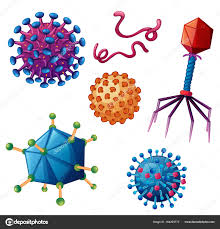
\includegraphics[width=0.9\textwidth]{Figure/virus.jpg}
\end{figure}}
\only<2>{\begin{figure}[ht]
    \centering
    \vspace{-0.5cm}
    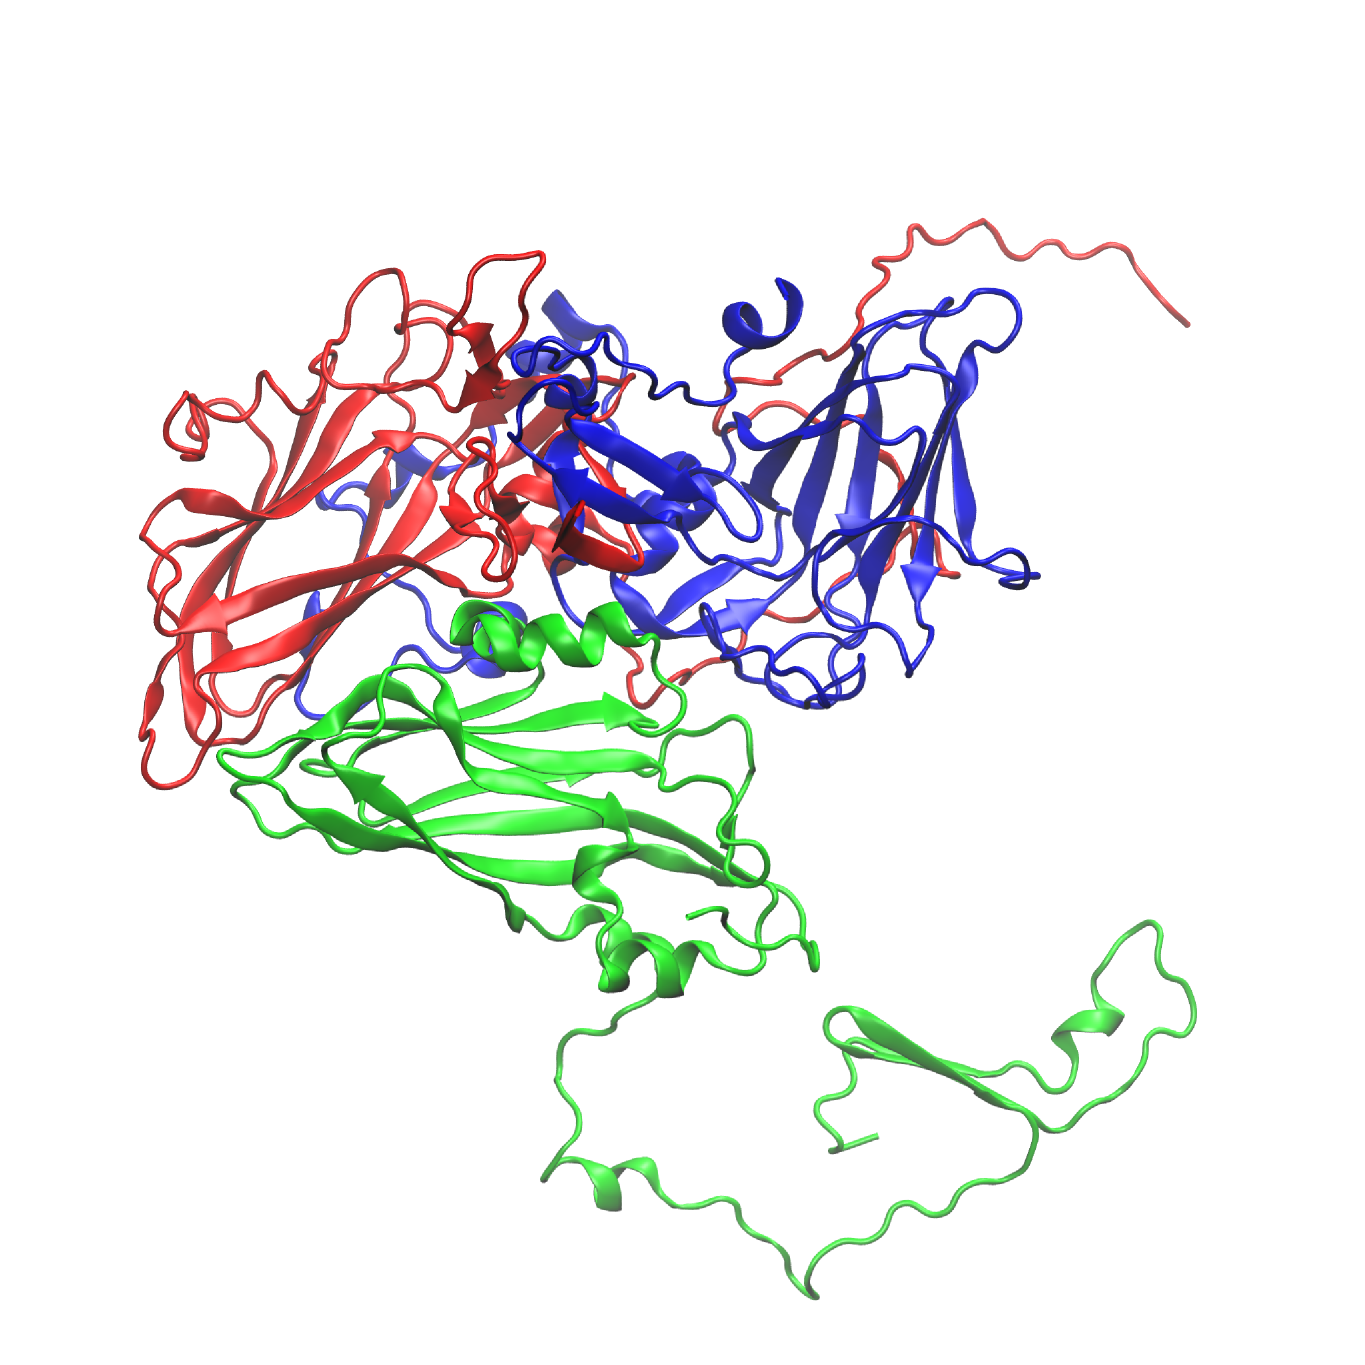
\includegraphics[width=0.8\textwidth]{Figure/TrV_Protomer.png}\\
    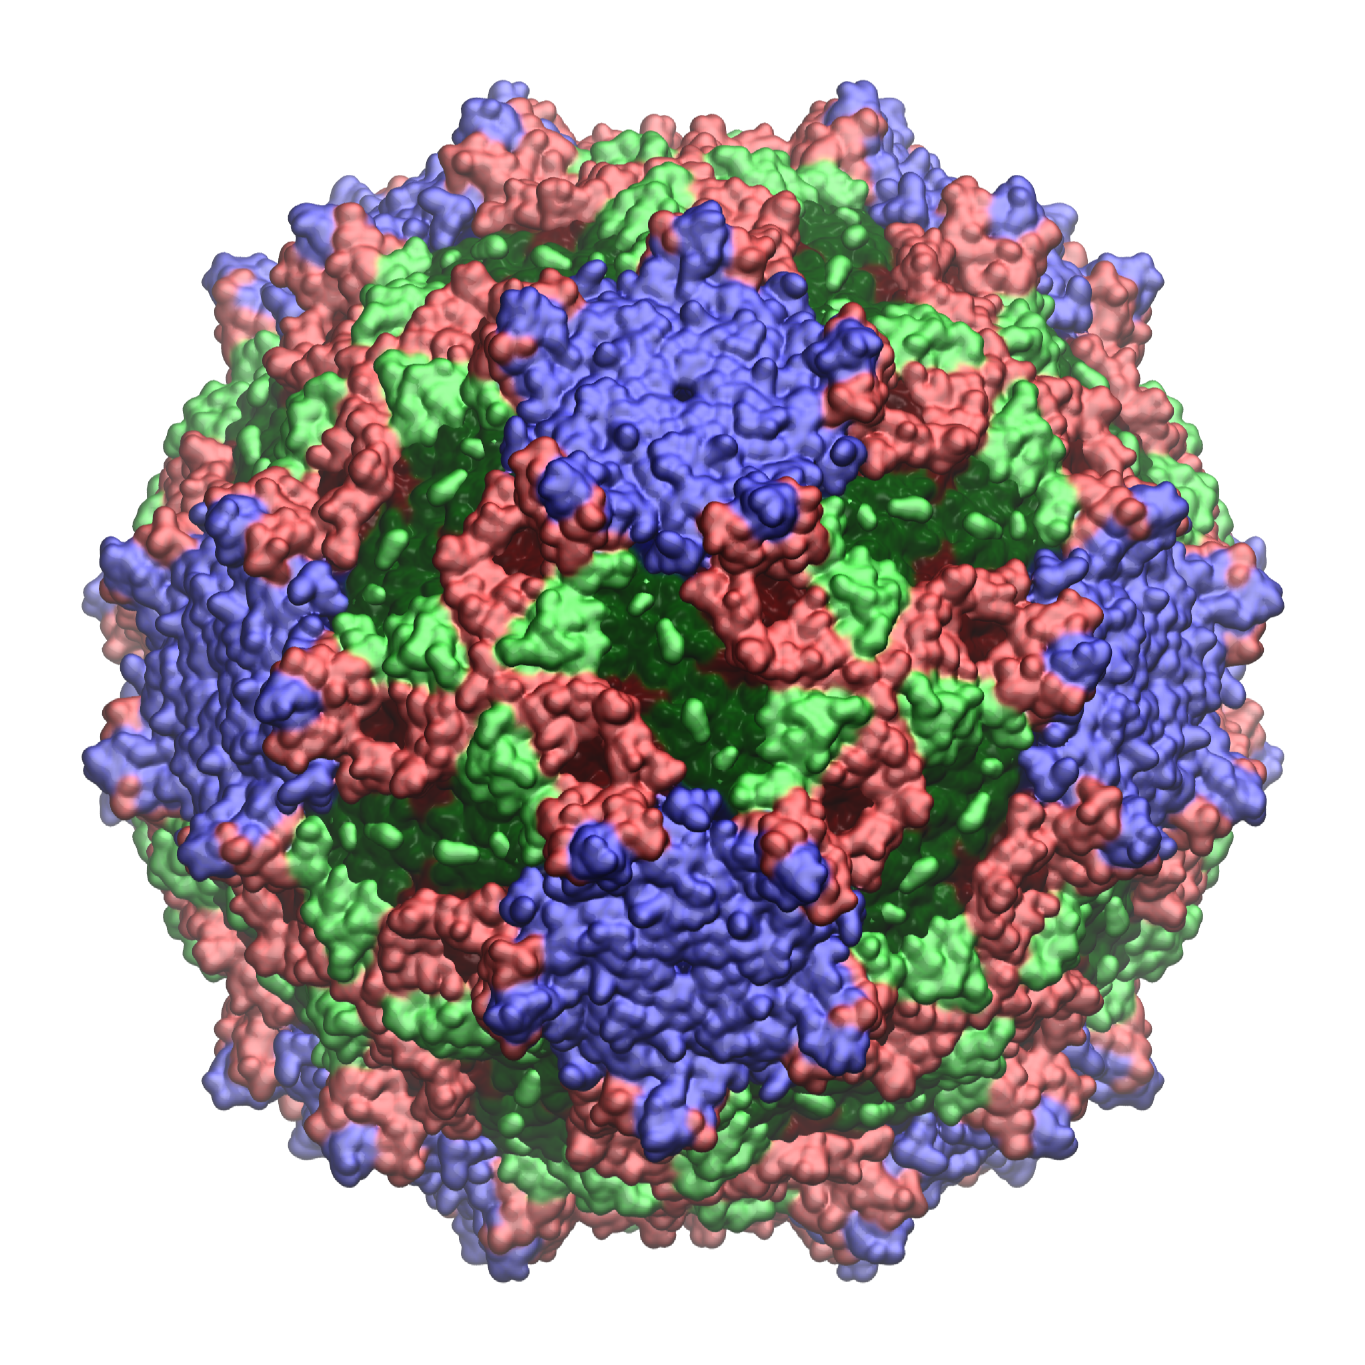
\includegraphics[width=0.8\textwidth]{Figure/TrV_Capsid.png}
\end{figure}}
\only<3-4>{\begin{figure}[ht]
    \centering
    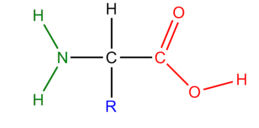
\includegraphics[width=0.9\textwidth]{Figure/aa.jpg}\\
    \end{figure}}
\only<5>{\begin{figure}
    \centering
    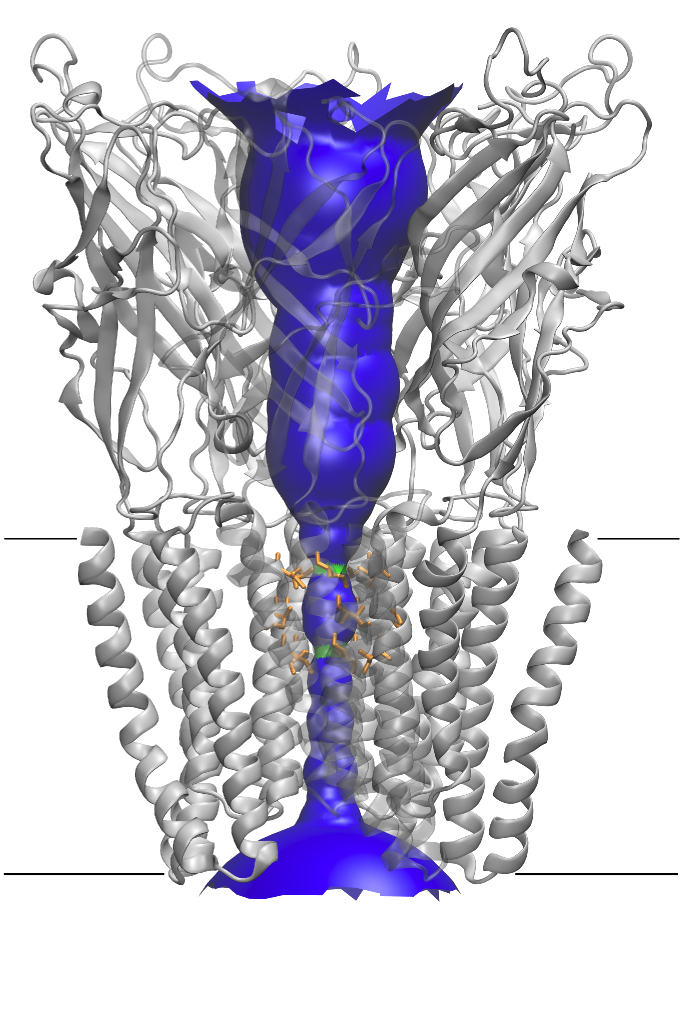
\includegraphics[width=0.9\textwidth]{Figure/GLIC.png}    
\end{figure}}
\end{minipage}

\begin{textblock*}{10cm}(0.14\textwidth,0.2\textheight)
\only<4>{
\begin{figure}
    \centering
    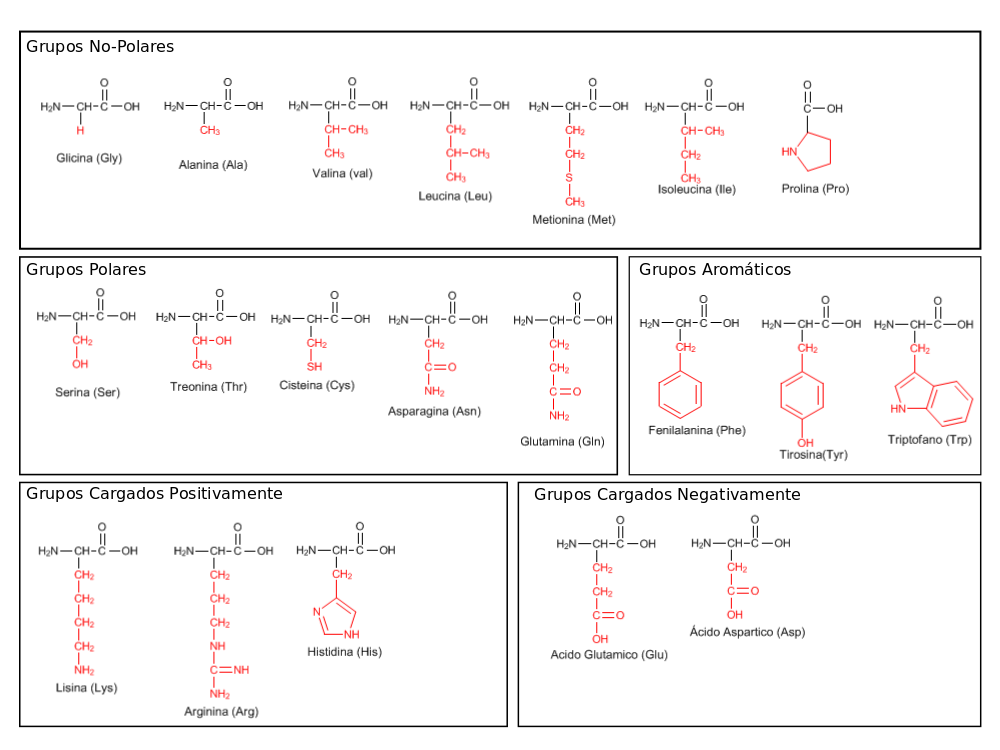
\includegraphics[width=0.9\textwidth]{Figure/aa2.png}
\end{figure}}
\end{textblock*}

\end{frame}

\begin{frame}[t]
%\vspace{-1cm}
\justifying
Los \alert{virus icosaédricos}, como los del género Picornavirales, poseen cápsides con gran simetría. Estas cápsides poseen varios ejes de simetría dobles, triples y \alert{quíntuples}. Particularmente, se ha propuesto que la cavidad presente en el \alert{eje de simetría quíntuple} podría ejercer un \alert{rol como canal de iones} (\textit{S. Kalko y A. Silva 1987}). Sin embargo, \alert{esta hipótesis \textbf{no} ha sido corroborada}.

\only<1>{
\begin{figure}[ht]
\centering
\hspace*{\fill}

\begin{subfigure}[t]{.46\textwidth}
  \centering
\begin{tikzpicture}
\node[anchor=center,inner sep=0,yshift=-0.2cm] at (0,0)
  {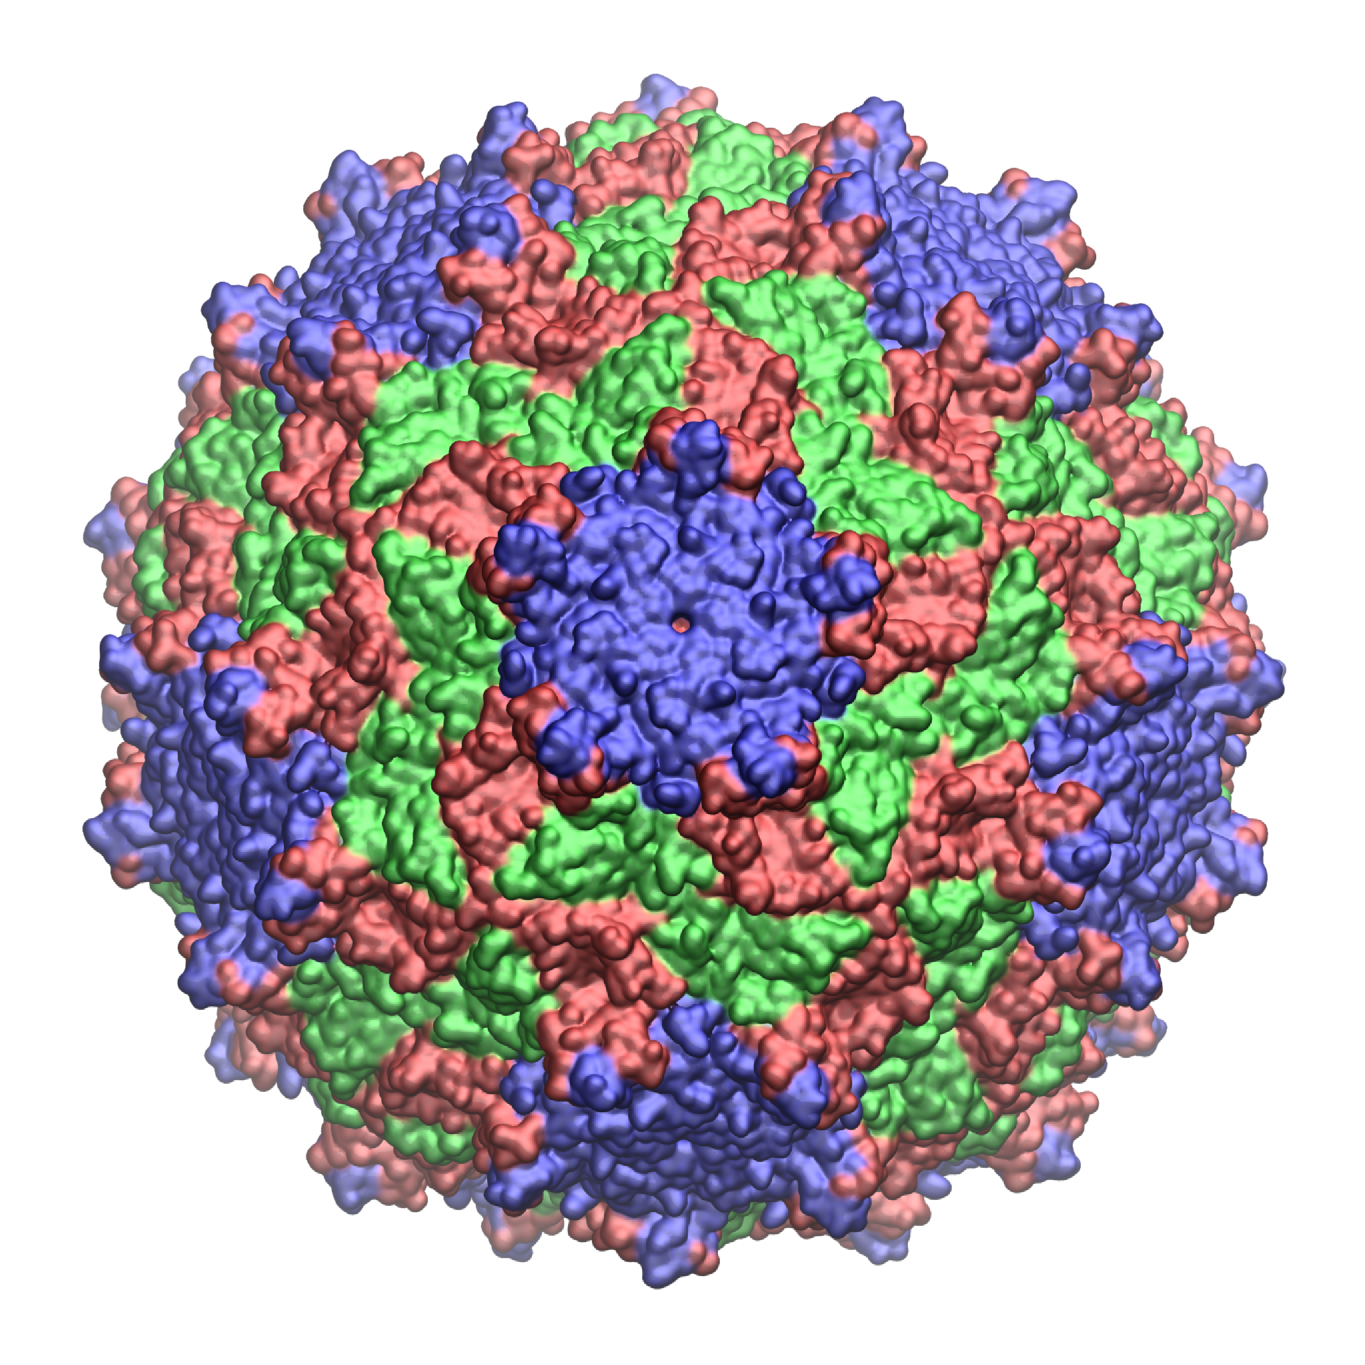
\includegraphics[width=1\textwidth]{Figure/TrV_Capsid_Ch4.png}};
\path (0+18:0.25cm) coordinate (P0);
\path (1*72+18:0.25cm) coordinate (P1);
\path (2*72+18:0.25cm) coordinate (P2);
\path (3*72+18:0.25cm) coordinate (P3);
\path (4*72+18:0.25cm) coordinate (P4);
\draw[,yellow,fill=yellow,ultra thick] (P0) -- (P1) -- (P2) -- (P3) -- (P4) -- cycle;
\path (0+30:0.25cm)+(0,1.3cm) coordinate (P1);
\path (1*120+30:0.25cm)+(0,1.3cm) coordinate (P2);
\path (2*120+30:0.25cm)+(0,1.3cm) coordinate (P3);
\draw[yellow,fill=yellow,ultra thick] (P1) -- (P2) -- (P3) -- cycle;
\coordinate (P0) at (-0.25,-1.1);
\coordinate (P1) at (0.25,-1.1);
\draw[yellow,fill=yellow,ultra thick] (P0) to [bend left=30] (P1);
\draw[yellow,fill=yellow,ultra thick] (P1) to [bend left=30] (P0);
\end{tikzpicture} 
\end{subfigure}
\hspace*{\fill}
\begin{subfigure}[t]{.46\textwidth}
  \centering
\begin{tikzpicture}
\node[anchor=center,inner sep=0] at (0,0)
  {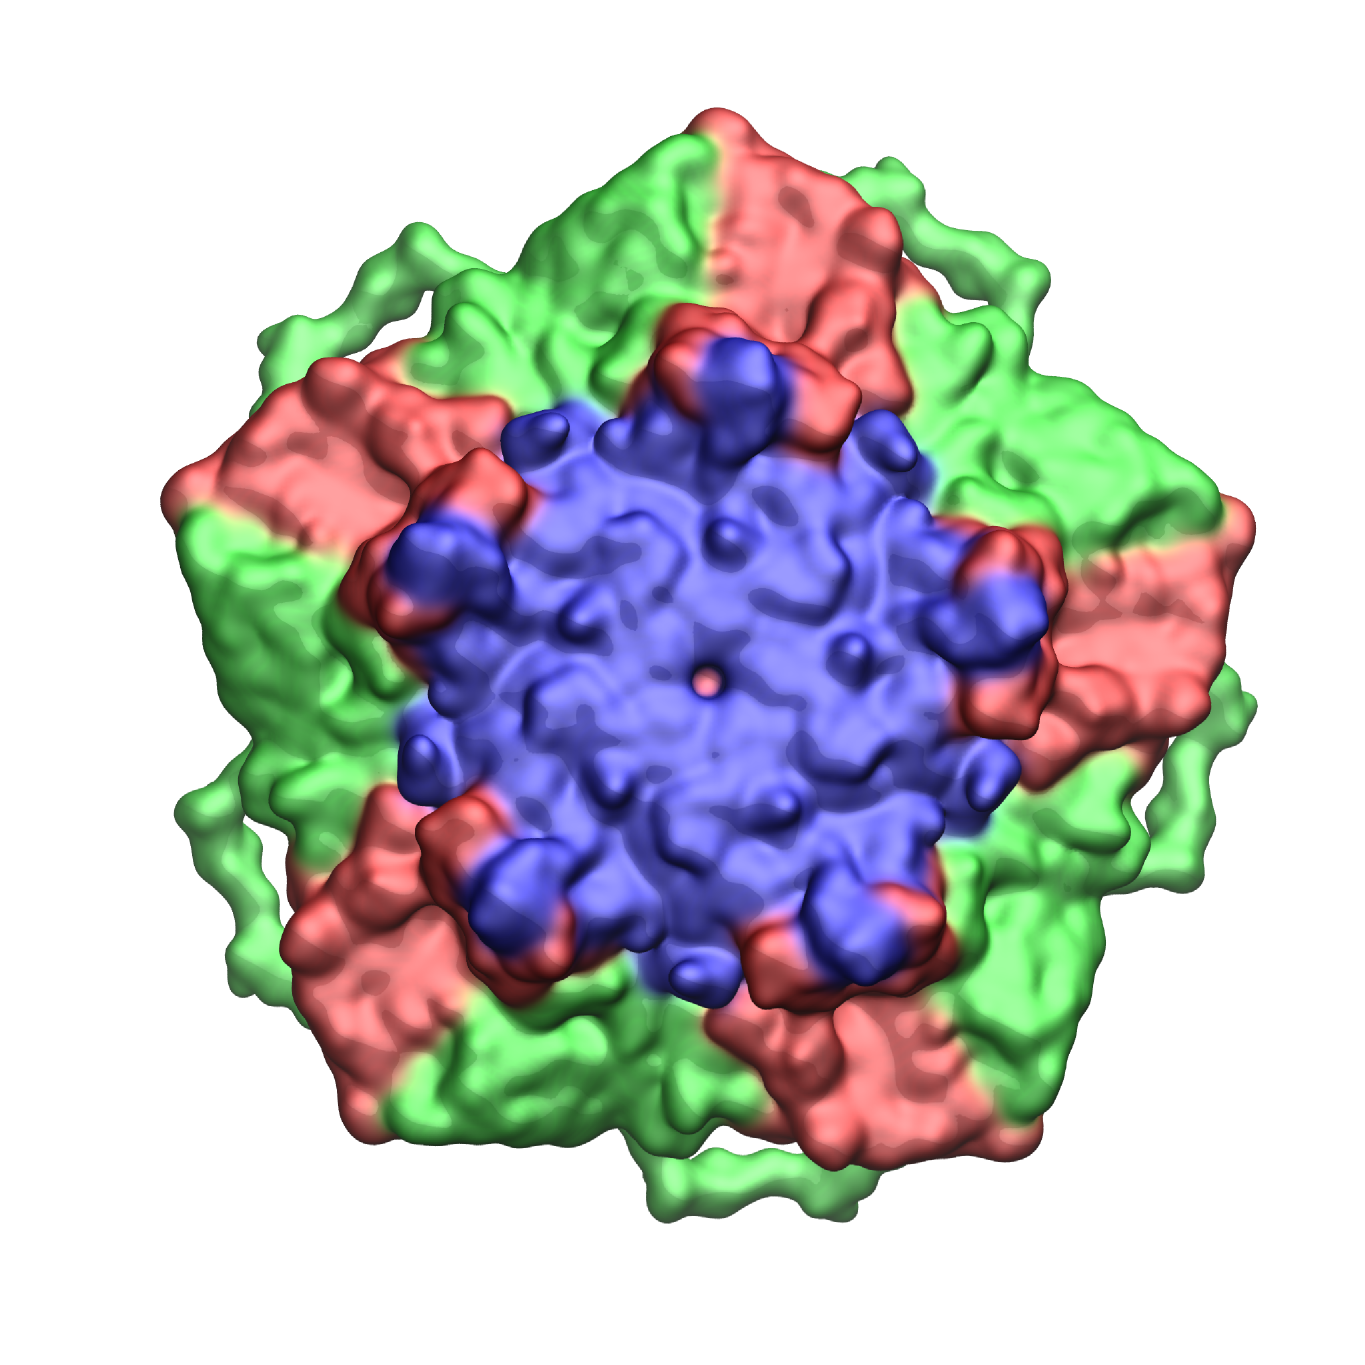
\includegraphics[width=1\textwidth]{Figure/TrV_Pentamer_Ch4.png}};
\path (0+18:0.25cm)+(0.1cm,0) coordinate (P0);
\path (1*72+18:0.25cm)+(0.1cm,0) coordinate (P1);
\path (2*72+18:0.25cm)+(0.1cm,0) coordinate (P2);
\path (3*72+18:0.25cm)+(0.1cm,0) coordinate (P3);
\path (4*72+18:0.25cm)+(0.1cm,0) coordinate (P4);
\draw[yellow,fill=yellow,ultra thick] (P0) -- (P1) -- (P2) -- (P3) -- (P4) -- cycle;
\path (0+30:0.25cm)+(0.15cm,2.2cm) coordinate (P1);
\path (1*120+30:0.25cm)+(0.15cm,2.2cm) coordinate (P2);
\path (2*120+30:0.25cm)+(0.15cm,2.2cm) coordinate (P3);
\draw[yellow,fill=yellow,ultra thick] (P1) -- (P2) -- (P3) -- cycle;
\coordinate (P0) at (-0.15,-1.8);
\coordinate (P1) at (0.35,-1.8);
\draw[yellow,fill=yellow,ultra thick] (P0) to [bend left=30] (P1);
\draw[yellow,fill=yellow,ultra thick] (P1) to [bend left=30] (P0);
\end{tikzpicture} 
\end{subfigure}
\hspace*{\fill}
\end{figure}
}

\only<2>{
\centering
\begin{figure}[ht]
  \centering
  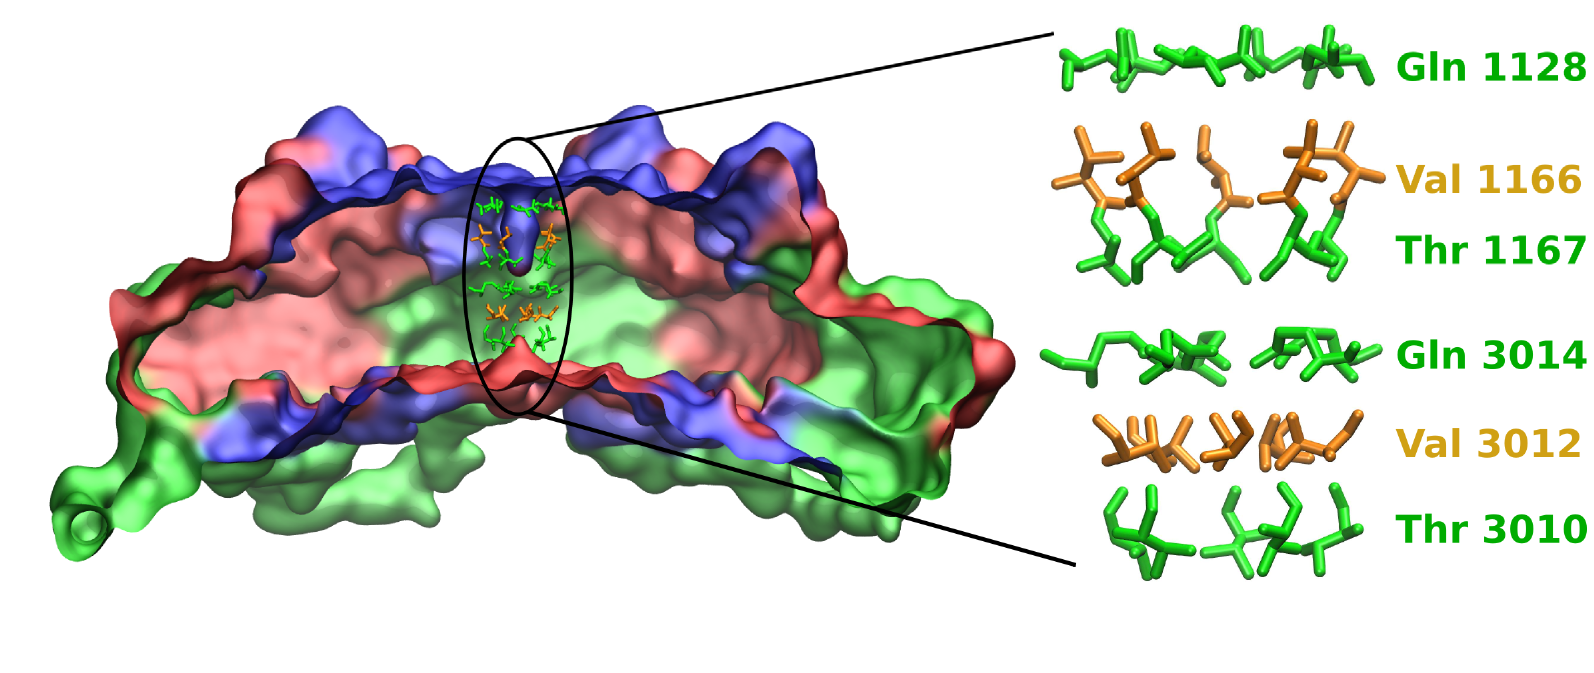
\includegraphics[width=1\textwidth]{Figure/TrV_Sideview_Pore.png}
\end{figure}
}

\end{frame}

%
% Objetivos
%

\subsection*{Objetivos}
\begin{frame}[t]{Objetivos}
\justifying
\begin{wrapfigure}{r}{0.4\textwidth}
\vspace{-0.5cm}
\Centering
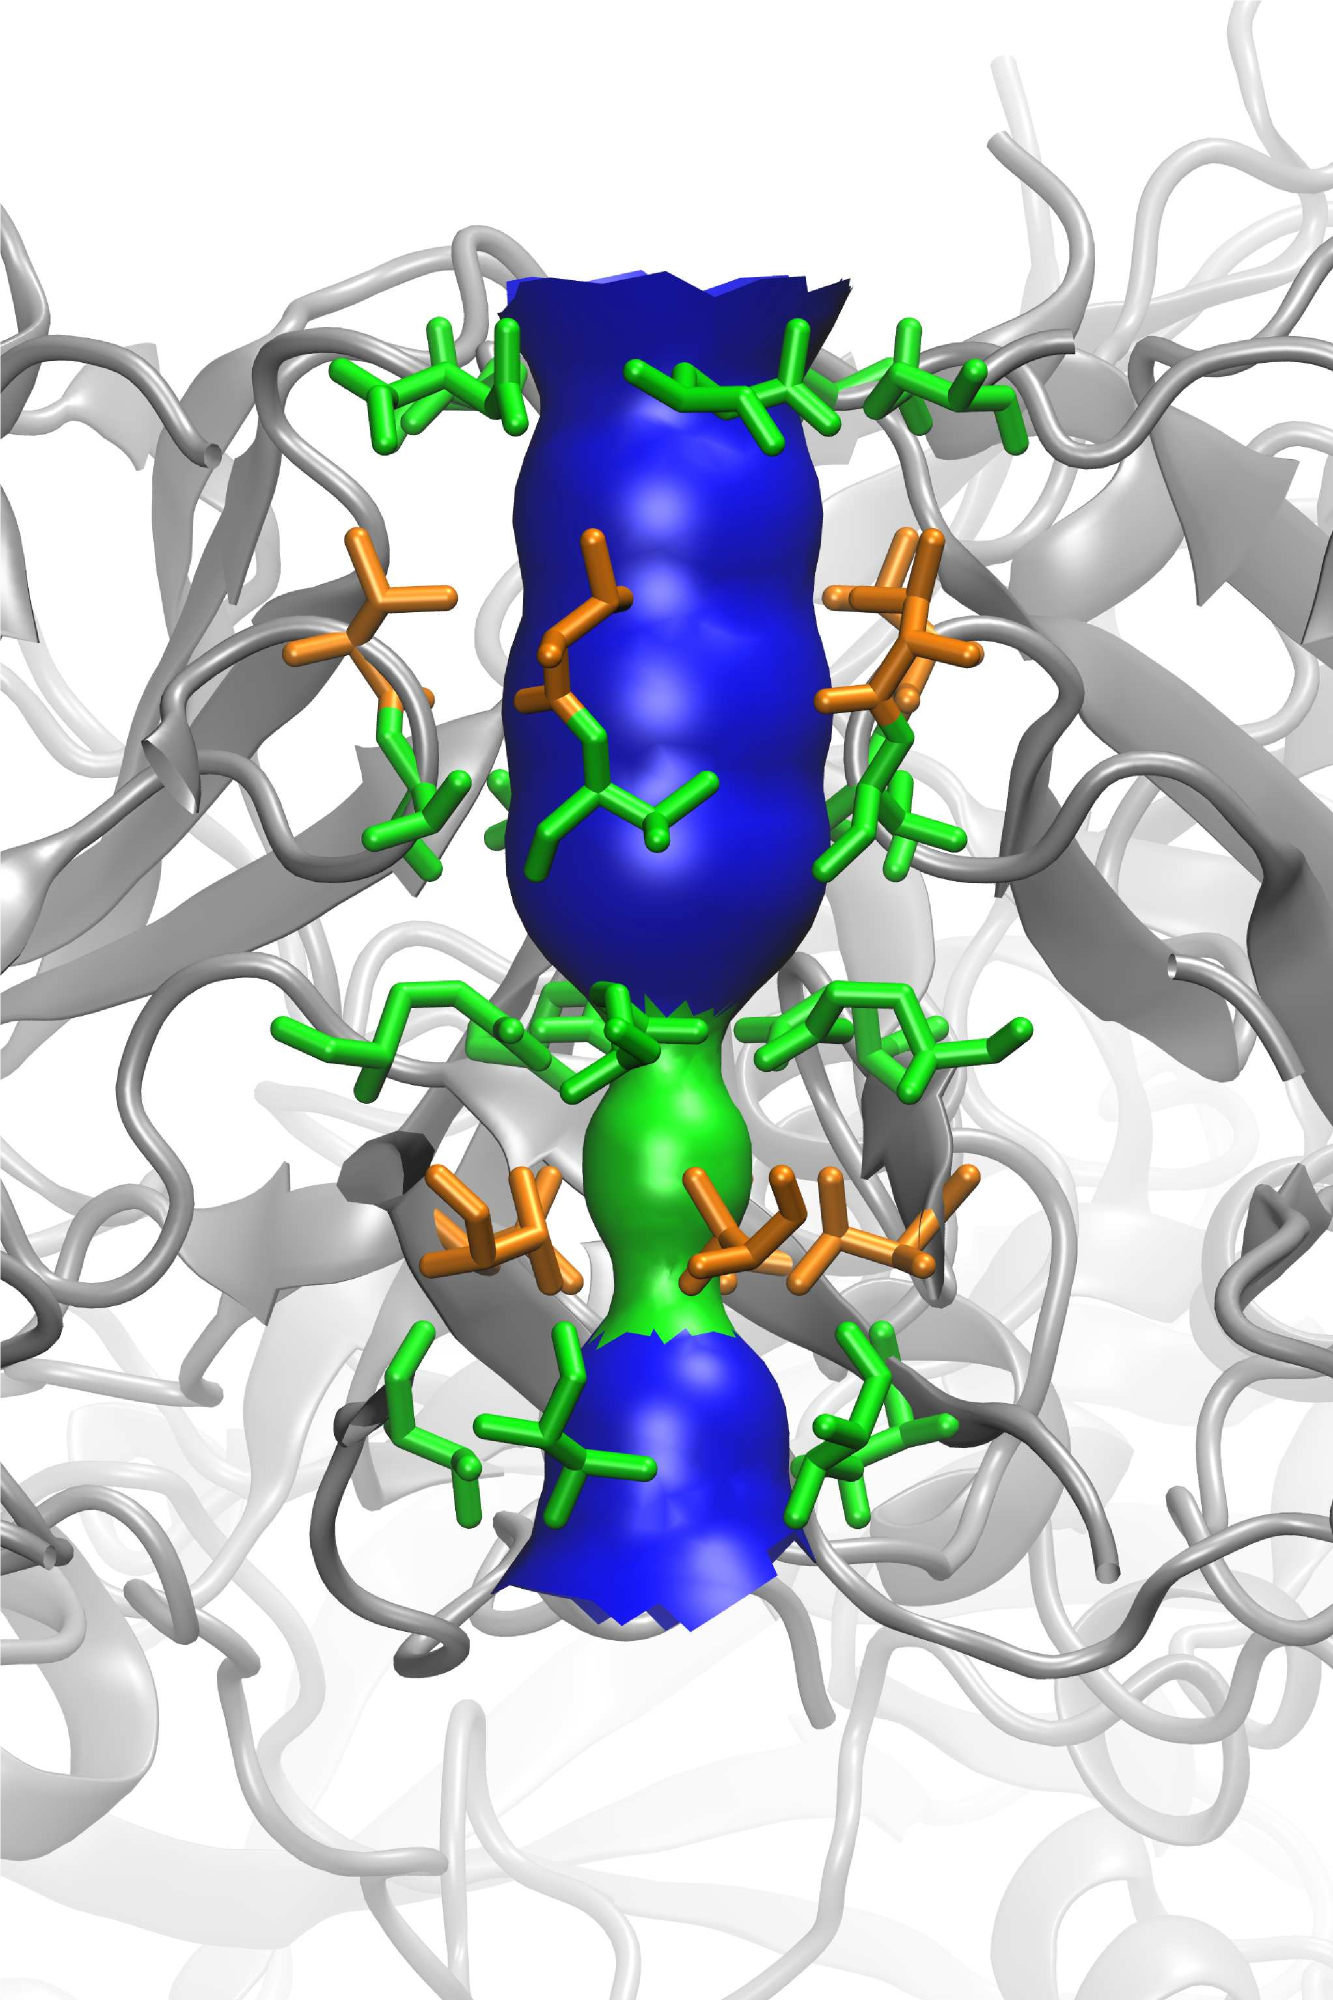
\includegraphics[width=0.35\textwidth]{Figure/TrV_Sideview_Pore_2.png}
\end{wrapfigure}

El objetivo de esta tesis es lograr \alert{determinar}, a partir de técnicas computacionales, el \alert{rol de la cavidad presente en el eje de simetría quíntuple} en el virus del Triatoma.
\begin{itemize}
\justifying
\item[$\bullet$] Determinar si el poro de TrV tiene función de canal.
\item[$\bullet$] Determinar si el poro posee algún mecanismo de regulación de su apertura.
\item[$\bullet$] Determinar que tipo de moléculas son capaces de atravesarlo.
\item[$\bullet$] Determinar similitudes y diferencias entre la estructura del eje quíntuple con la estructura de otros virus pertenecientes al género.
\end{itemize}

\end{frame}

% These three lines create an automatically generated table of contents.
\begin{frame}[t]
  \tableofcontents
\end{frame}

\AtBeginSection[]{        % Frame added before each section
  \frame<handout:0>{
    \tableofcontents[current]                   % Highlight current section/subsection
  }}

%
% Introducción
%

\section{Introducción}
\subsection{Virus del Triatoma}
\begin{frame}{Virus del Triatoma - TrV}
    \begin{columns}
    \begin{column}{0.2\textwidth}
    \large
    \vspace{0.1cm}
    \textit{Picornavirales}
    \end{column}
    \hspace{-1.5cm}
    \begin{column}{0.1\textwidth}
    \left \{
    \begin{tabular}{l}
    Picornavirus\\
    Dicistrovirus $\longrightarrow$\\
    Secovirus
    \end{tabular}
    \right.
    \end{column}
    \begin{column}{0.3\textwidth}
    \tikzmarkin<2->[set fill color=green!10, set border color=green]{f1}  
    \tikz[remember picture,baseline,inner sep=1ex]\node[anchor=base](n1){Triatoma Virus.}; \tikzmarkend{f1}
    \end{column}
    \end{columns}
    
    \vfill
    
    \onslide<2->{
    $\bullet$  \tikzmarkin<2->[set fill color=green!10, set border color=green]{f2} \tikz[remember picture,baseline,inner sep=0]\node[anchor=base](n2){Patógeno Natural}; \tikzmarkend{f2}
    del \textit{Triatoma Infestans}, insecto mejor conocido en América Latina como 
    \tikzmarkin<3->[set fill color=red!10, set border color=red]{f3} 
    \tikz[remember picture,baseline,inner sep=1ex]\node[anchor=base](n3){Vinchuca.};
    \tikzmarkend{f3}\\
    }

    \vfill
    
    \onslide<3->{
    $\bullet$ Principal 
    \tikzmarkin<3->[set fill color=red!10, set border color=red]{f4} 
    \tikz[remember picture,baseline,inner sep=1ex]\node[anchor=base](n4){vector};
    \tikzmarkend{f4} de la \textit{Trypanosomiasis Americana} o Mal de Chagas.\\
    }

\begin{tikzpicture}[remember picture,overlay]
\draw<2->[thick,green,->] (n1) -- (n2);
\end{tikzpicture}
\begin{tikzpicture}[remember picture,overlay]
\draw<3->[thick,red,->] (n3) -- (n4);
\end{tikzpicture}
    
\end{frame}

\subsection{Dinámica Molecular}
\begin{frame}[t]{Dinámica Molecular}

Integrador de Leap-Frog:
\begin{align*}
&x(t+\Delta t) = x(t) + v(t+\frac{1}{2}\Delta t){\Delta t} \nonumber \\
&v(t+\frac{1}{2}\Delta t) = v(t-\frac{1}{2}\Delta t) + a\Delta t
\end{align*}

\invisible<-1>{
Campo de Fuerzas:
\begin{multline*}
V = \tikzmarkin<3->[set fill color=green!10, set border color=green!30!black!80]{cc}(0,-0.4)(0,0.4) \sum\limits_{enlaces} \frac{k_{b,i}}{2} (l_i-l_{i0})^2 \tikzmarkend{cc}
+ \tikzmarkin<4->[set fill color=green!10, set border color=green!30!black!80]{dd}(0,-0.4)(0,0.4) \sum\limits_{angulos} \frac{k_{\theta,i}}{2} (\theta_i-\theta_{i,0})^2 \tikzmarkend{dd}
+ \tikzmarkin<5->[set fill color=green!10, set border color=green!30!black!80]{ee}(0,-0.4)(0,0.4) \sum\limits_{torsiones} \frac{\nu_n}{2} (1+cos(n\omega-\gamma)) \tikzmarkend{ee} \\
+ \sum\limits_{i=1} \sum\limits_{j=i+1} (
\tikzmarkin<6->[set fill color=blue!10, set border color=blue]{aa}(0,-0.4)(0,0.4) 4\epsilon[(\frac{\sigma_{ij}}{r_{ij}})^{12}-(\frac{\sigma_{ij}}{r_{ij}})^6] \tikzmarkend{aa}
+ \tikzmarkin<7->[set fill color=red!10, set border color=red]{bb}(0,-0.4)(0,0.4) \frac{q_iq_j}{4\pi\epsilon_0r_{ij}} \tikzmarkend{bb}
)
\end{multline*}
}

\begin{minipage}{0.4\textwidth}
\invisible<-1>{
\vspace{-0.5cm}
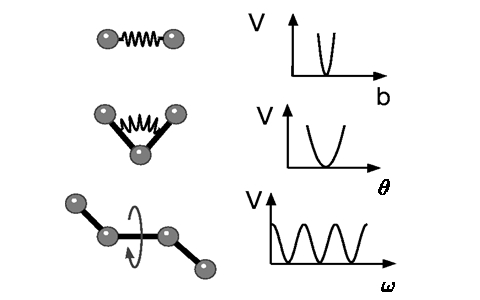
\includegraphics[width=\textwidth]{Figure/ff.jpg}
}
\end{minipage}
\begin{minipage}{0.59\textwidth}
\invisible<-2>{
  \vspace{-0.5cm}
  \begin{center}
  \begin{tabular}{cl}
  \onslide<3->{\color{green!30!black!80} Potencial enlazante: enlaces} \\
  \onslide<4->{\color{green!30!black!80} Potencial enlazante: ángulos} \\
  \onslide<5->{\color{green!30!black!80} Potencial enlazante: torsiones} \\
  \onslide<6->{\color{blue} Potencial de Lennard-Jones} \\
  \onslide<7->{\color{red} Potencial Coulombiano} 
  \end{tabular}
  \end{center}
}
\end{minipage}
\end{frame}

\subsection{Campos de Fuerza}
\begin{frame}[t]{Campos de Fuerza}
\justifying


\begin{wrapfigure}{r}{0.7\textwidth}
\begin{figure}[ht]
\centering
\hspace*{\fill}
\begin{subfigure}[t]{.32\textwidth}
  \vspace{-1cm}
  \centering
  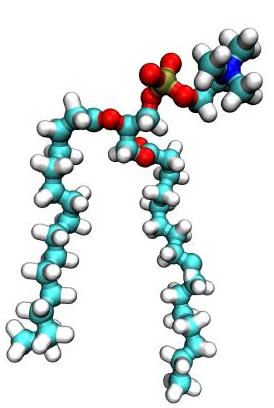
\includegraphics[width=0.75\textwidth]{Figure/FF-AA.png}
\end{subfigure}
\onslide<2->{
\hspace*{\fill}
\begin{subfigure}[t]{.32\textwidth}
  \vspace{-1cm}
  \centering
  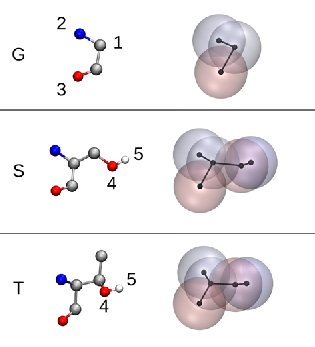
\includegraphics[width=0.8\textwidth]{Figure/FF-CG.png}
\end{subfigure}
}
\hspace*{\fill}
\onslide<3->{
\begin{subfigure}[t]{.32\textwidth}
%   \vspace{-0.1cm}
  \centering
  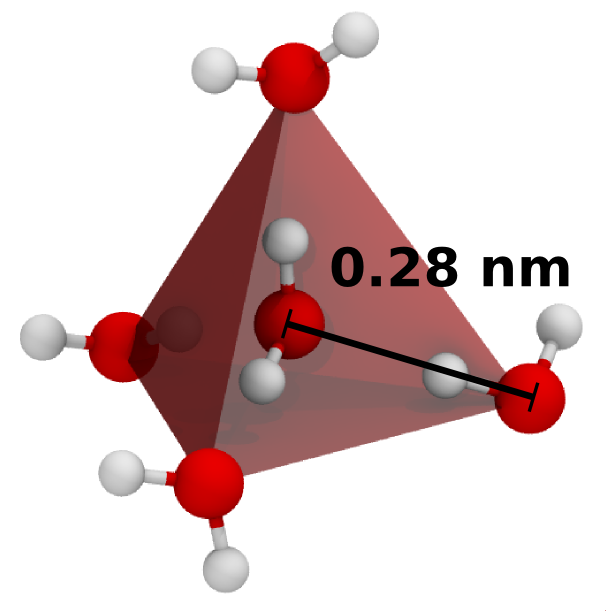
\includegraphics[width=0.7\textwidth]{Figure/FF-wt4A.png}
\end{subfigure}
\hspace*{\fill}
\begin{subfigure}[t]{.32\textwidth}
%   \vspace{-0.1cm}
  \centering
  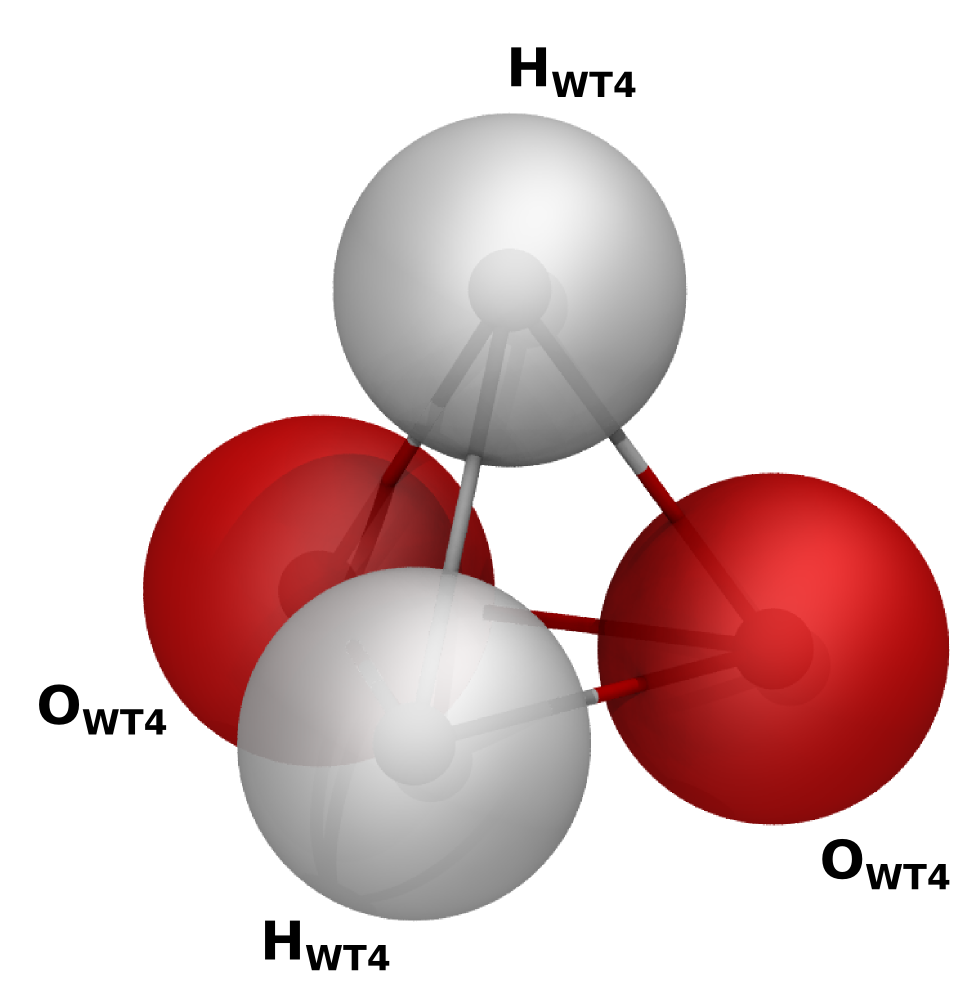
\includegraphics[width=0.7\textwidth]{Figure/FF-wt4B.png}
\end{subfigure}
}
\hspace*{\fill}
\end{figure}
\end{wrapfigure}


\textbf{Atomísticos}
\begin{enumerate}
    \item \tikzmarkin<4->[set fill color=red!10, set border color=red]{a} GROMOS \tikzmarkend{a}
    \item AMBER
    \item CHARMM
    \item OPLS
\end{enumerate}
\vspace{0.5cm}

\onslide<2->{
\textbf{Grano Grueso}
\begin{enumerate}
    \item \tikzmarkin<4->[set fill color=red!10, set border color=red]{b} Sirah \tikzmarkend{b}
    \item Martini
\end{enumerate}
\vspace{0.5cm}
}

\onslide<3->{
\textbf{Modelos de Agua}
\begin{enumerate}
    \item \tikzmarkin<4->[set fill color=red!10, set border color=red]{c} SPC \tikzmarkend{c}
    \item SPC/e
    \item TIP3P
    \item \tikzmarkin<4->[set fill color=red!10, set border color=red]{d} WT4 y WLS \tikzmarkend{d}
\end{enumerate}
}

\end{frame}

\begin{frame}[t]{Dinámica Molecular}
\onslide<1->\centering \large{\textbf{Gromacs}} \\
\only<1>{
\begin{figure}
    \centering
    
\includegraphics[width=0.6\textwidth]{Figure/GROMACS.png}
\end{figure}}
\hspace{-0.4cm}
\begin{minipage}[t]{0.38\textwidth}
\begin{itemize}
    \setlength\itemsep{1em}
    \item<2-> Caja de simulación: \textbf{Dodecaédrico rómbico}
    \item<3-> Condiciones de borde Periódicas.
    \item<4-> Termostato:
    \tikzmarkin<4>[set fill color=red!10, set border color=red]{eq11}
    Berendsen \tikzmarkend{eq11} o
    \tikzmarkin<4>[set fill color=blue!10, set border color=blue]{eq22}
    v-rescale. \tikzmarkend{eq22} 
    \item<4-> Barostato:
    \tikzmarkin<4>[set fill color=green!10, set border color=green]{eq33}
    Berendsen \tikzmarkend{eq33} o
    \tikzmarkin<4>[set fill color=violet!10, set border color=violet]{eq44}
    Parrinello-Rahman. \tikzmarkend{eq44}
\end{itemize}
\end{minipage}
\hspace{0.4cm}
\begin{minipage}[t]{0.5\textwidth}
\vspace{1cm}
\only<2>{
\begin{figure}[ht]
  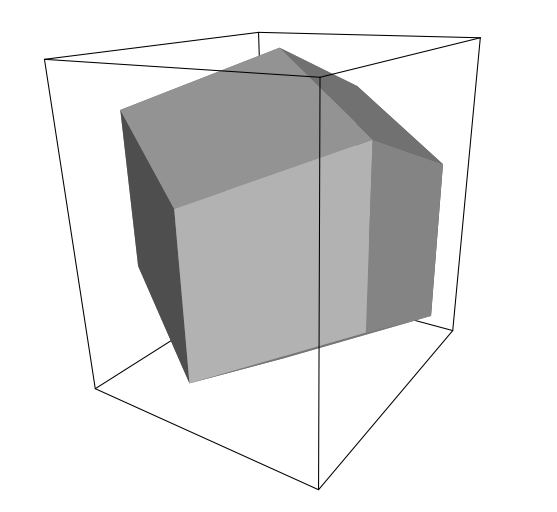
\includegraphics[width=0.8\textwidth]{Figure/box.png}
\end{figure}}
\only<3>{
\begin{figure}[ht]
  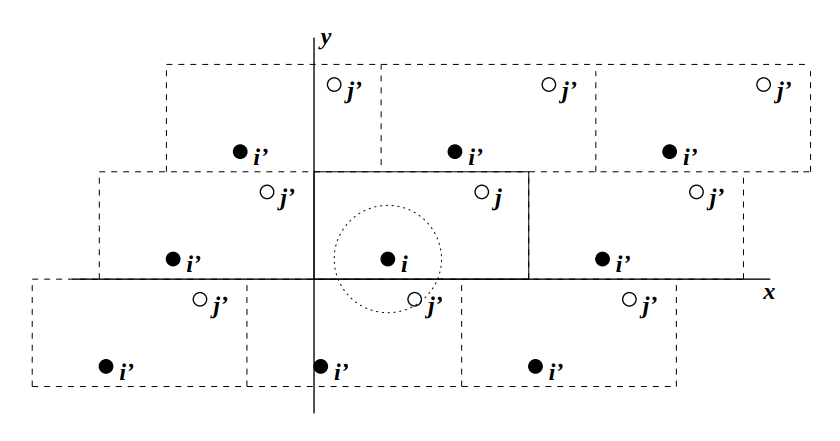
\includegraphics[width=0.8\textwidth]{Figure/pbc.png}
\end{figure}}
\only<4>{
\begin{equation*}
\tikzmarkin<4>[set fill color=red!10, set border color=red]{eq1}(0,-0.4)(0,0.6)
\frac{dT(t)}{dt}=\frac{1}{\tau}(T_{ba\tilde{n}o}-T(t))
\tikzmarkend{eq1}
\end{equation*}
\vspace{0.1cm}
\begin{equation*}
\tikzmarkin<4>[set fill color=blue!10, set border color=blue]{eq2}(0,-0.4)(0,0.6)
dK=\frac{dt}{\tau}(K_{ba\tilde{n}o}-K)+2\sqrt{\frac{KK_{ba\tilde{n}o}}{N_l}\frac{dW}{\sqrt{\tau}}}
\tikzmarkend{eq2}
\end{equation*}
\vspace{0.1cm}
\begin{equation*}
\tikzmarkin<4>[set fill color=green!10, set border color=green]{eq3}(0,-0.4)(0,0.6)
\frac{dP(t)}{dt}=\frac{1}{\tau}(P_{ba\tilde{n}o}-P(t))
\tikzmarkend{eq3}
\end{equation*}
\vspace{0.1cm}
\begin{equation*}
\tikzmarkin<4>[set fill color=violet!10, set border color=violet]{eq4}(0,-0.4)(0,0.6)
\frac{d\bm{b}^2}{dt^2}=V\bm{W}^{-1}\bm{b}'^{-1}(P-P_0)
\tikzmarkend{eq4}
\end{equation*}
}
\end{minipage}
\end{frame}

%
% Poro en el eje quíntuple de TrV
%

\section{Puerta Hidrofóbica}
\subsection{Poro en el Eje Quíntuple de TrV}
\begin{frame}[t]{Poro en el Eje Quíntuple de TrV}
\begin{minipage}{0.4\textwidth}
\justifying
\begin{enumerate}[$\bullet$]
\item Estudio de la hidratación.
\item Dinámica Molecular a multiescala.
\item Proteína a nivel de detalle atómico.
\item Aguas periféricas a nivel de grano-grueso (Coarse-Grain).
\end{enumerate}
\end{minipage}
\hfill
\begin{minipage}{0.59\textwidth}
\onslide<2->{
\textbf{Protocolo}
\begin{itemize}
    \item Minimización de Energia: Steep Descent o Conjugate Gracients.
    \item Restricción de Posiciones: proteína fijas y aguas libres.
    \item Termalización: 1 ns de 100 K a 310 K.
    \item Simulaciones de Producción: hasta 100 ns.
\end{itemize}
}
\end{minipage}
\vspace{0.4cm}
\begin{center}
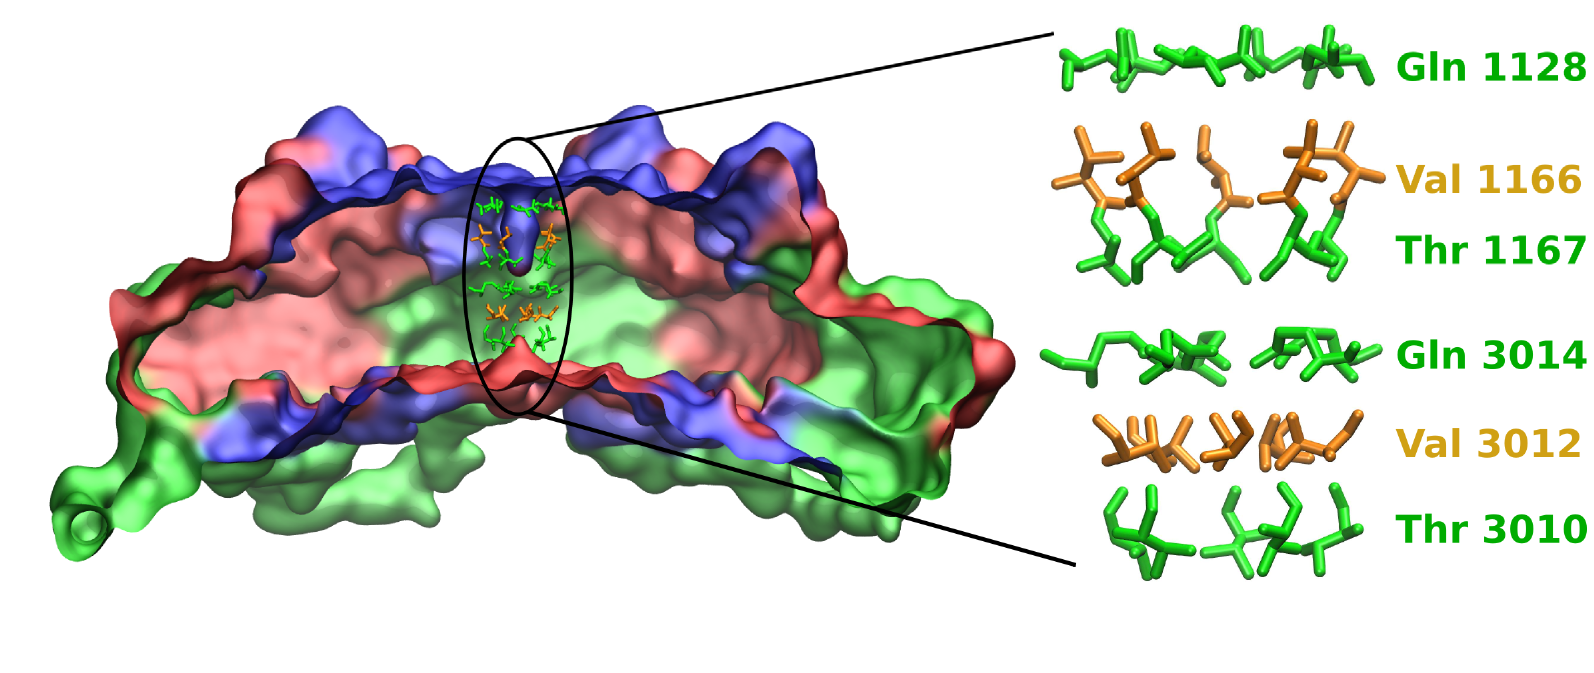
\includegraphics[width=0.8\textwidth]{Figure/TrV_Sideview_Pore.png}
    
\end{center}
\end{frame}

\subsection{Sistema a Simular}
\begin{frame}[t]{Sistema a Simular}

\begin{figure}[ht]
\vspace{-0.4cm}
\centering
\hspace*{\fill}
\begin{subfigure}[t]{.48\textwidth}
  \centering
  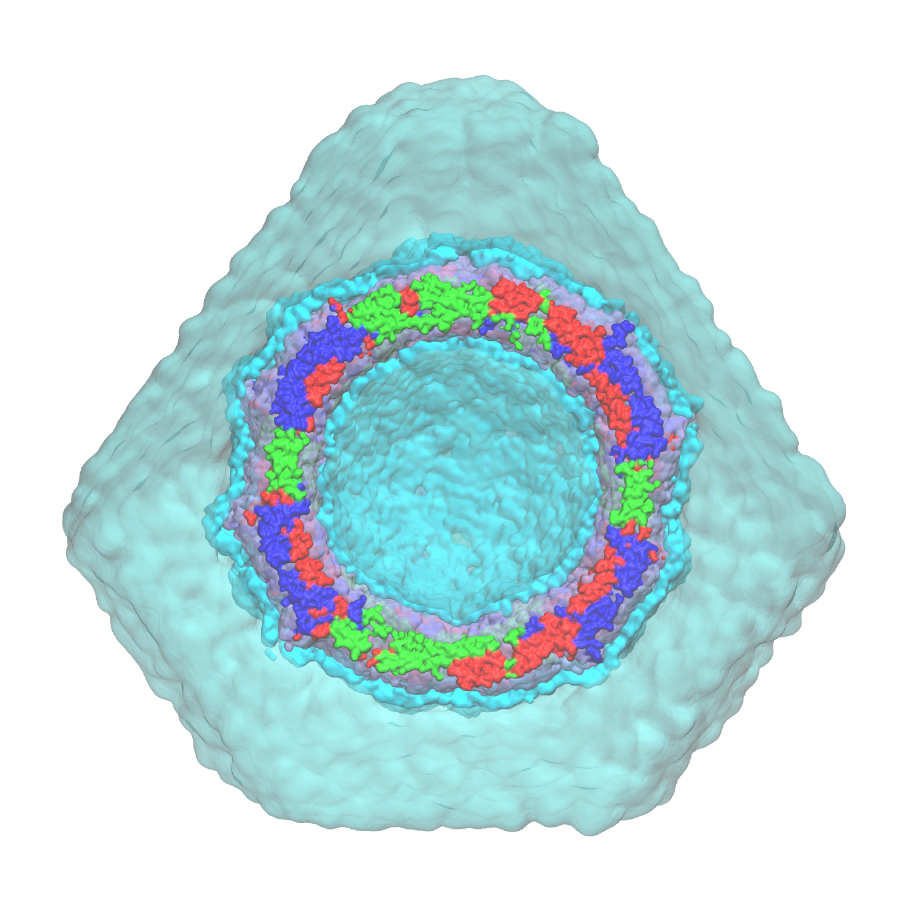
\includegraphics[width=1\textwidth]{Figure/TrV_Capsid_WaterBox.png}
  \vspace{-1cm}
  \caption*{
  \tikzmarkin<1->[set fill color=red!10, set border color=red, fill opacity=0.5]{ss1}(0,-0.2)(-0.6,0.3)
  \footnotesize{Atomístico $\sim3.300.000$ partículas(?) \\ Multiescala $\sim1.300.000$ partículas($\sim1\sfrac{ns}{d\acute{\imath}a}$)}
  \tikzmarkend{ss1}}
  \label{fig:trv_capsid_waterbox}
\end{subfigure}
\hspace*{\fill}
\begin{subfigure}[t]{.48\textwidth}
  \centering
  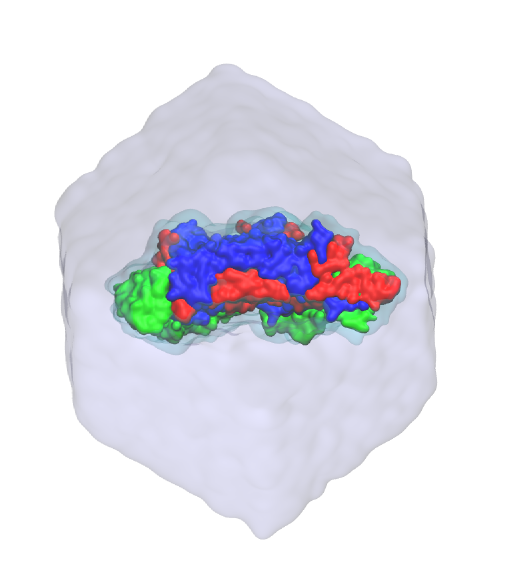
\includegraphics[width=1\textwidth]{Figure/TrV_Pentamer_WaterBox.png}
  \vspace{-1cm}
  \caption*{
  \tikzmarkin<1->[set fill color=red!10, set border color=red, fill opacity=0.5]{ss2}(0,-0.2)(-0.1,0.3)
  \footnotesize{Atomístico $\sim900.000$ partículas($\sim2\sfrac{ns}{d\acute{\imath}a}$) \\ Multiescala $\sim170.000$ partículas($\sim10\sfrac{ns}{d\acute{\imath}a}$)}
  \tikzmarkend{ss2}}
  \label{fig:trv_pentamer_waterbox}
\end{subfigure}
\hspace*{\fill}
%\vspace{-10mm}
\caption*{ Corte transversal del sistema de simulación, (a) cápside completa y (b) pentámero aislado. En azul, verde y rojo las superficies de las proteínas virales VP1, 2 y 3. Seguido de las capas de solvente SPC, WT4 y WLS representadas como superficies transparentes.}%
\end{figure}
\end{frame}

\subsection{Resultados - TrV Wild-Type}
\begin{frame}[t]{Resultados - TrV Wild-Type}
\begin{figure}[ht]
  \centering
  \vspace{-0.25cm}
  
  \begin{tikzpicture}
    \node[anchor=south west,inner sep=0] at (0,0)
    {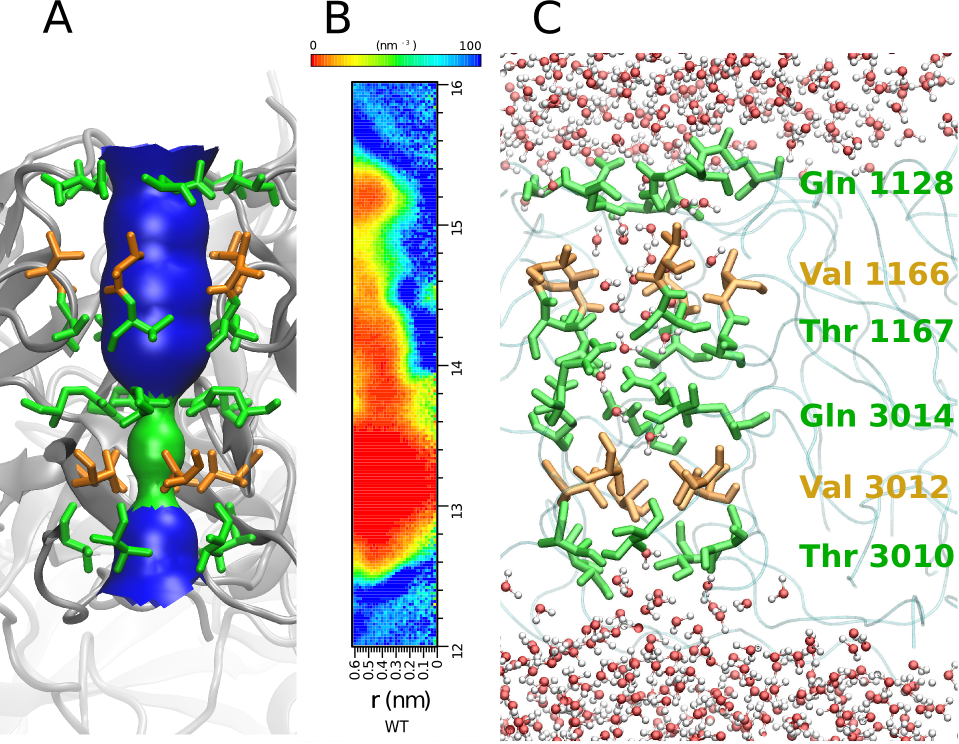
\includegraphics[height=6.3cm,keepaspectratio]{Figure/TrV_WT_Dens.png}};
    % \draw<3,5>[violet,ultra thick,rounded corners] (0.0,2.6) rectangle (7.0,3.0);
    \draw<2>[violet,ultra thick,rounded corners] (0.0,1.8) rectangle (8.2,2.6);
    \end{tikzpicture} \\
  \caption*{(A) Radio del poro. (B) Mapa de densidad de moléculas de agua. \\ (C) Vista lateral del poro de TrV.} %
\end{figure}
\end{frame}

\subsection{Resultados - TrV Mutación Valina por Serina}
\begin{frame}[t]{Resultados - TrV Mutación Valina por Serina}

\begin{figure}[ht]
  \centering
  \vspace{-0.25cm}
     \begin{tikzpicture}
    \node[anchor=south west,inner sep=0] at (0,0)
    {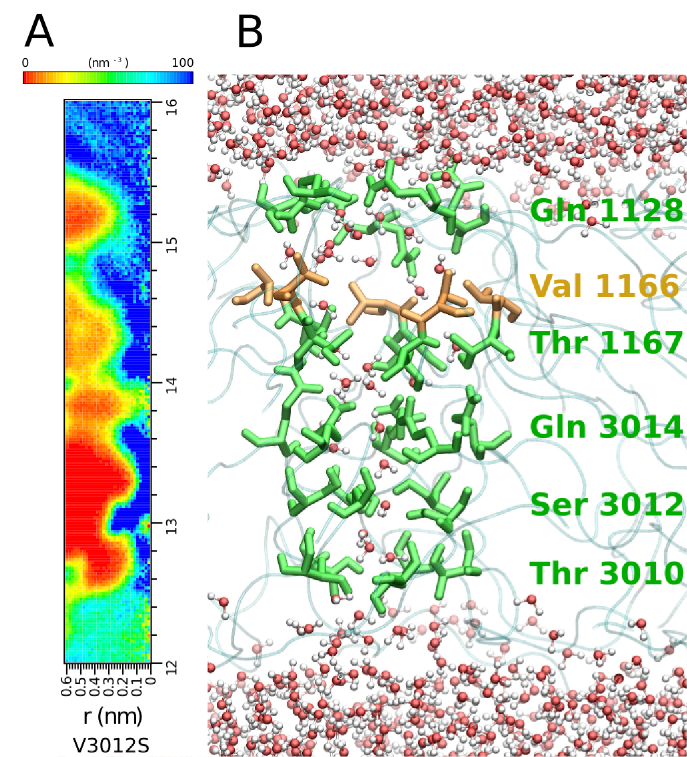
\includegraphics[height=6.3cm,keepaspectratio]{Figure/TrV_VS_Dens.png}};
    % \draw<3,5>[violet,ultra thick,rounded corners] (0.0,2.6) rectangle (7.0,3.0);
    \draw<2>[violet,ultra thick,rounded corners] (0.0,1.8) rectangle (6.0,2.4);
    \end{tikzpicture} \\
  \caption*{ (A) Mapa de densidad de moléculas de agua. (B) Vista lateral del poro de TrV mutado.}%
\end{figure}

\end{frame}

\subsection{Conclusión I}
\begin{frame}{Conclusión I}
\begin{itemize}
    \item Se observa la \alert{existencia de un poro en el eje quíntuple de TrV} capaz de comunicar el medio interior del virus con su exterior.\vfill
    \item Se observa la presencia de una \alert{puerta hidrofóbica} ubicada a la altura de las Valinas 3012.\vfill
    \item Estas características han sido observadas anteriormente en membranas celulares pero por \alert{primera vez en cápsides virales}.
\end{itemize}
\end{frame}

%
% Apertura de la Puerta
%

\section{Apertura de la Puerta}
\subsection{Densidad Electrónica Desconocida}
\begin{frame}{Mapa de Densidad Electrónica}
\centering
\begin{tikzpicture}
\node[anchor=south west,inner sep=0] at (0,0)
    {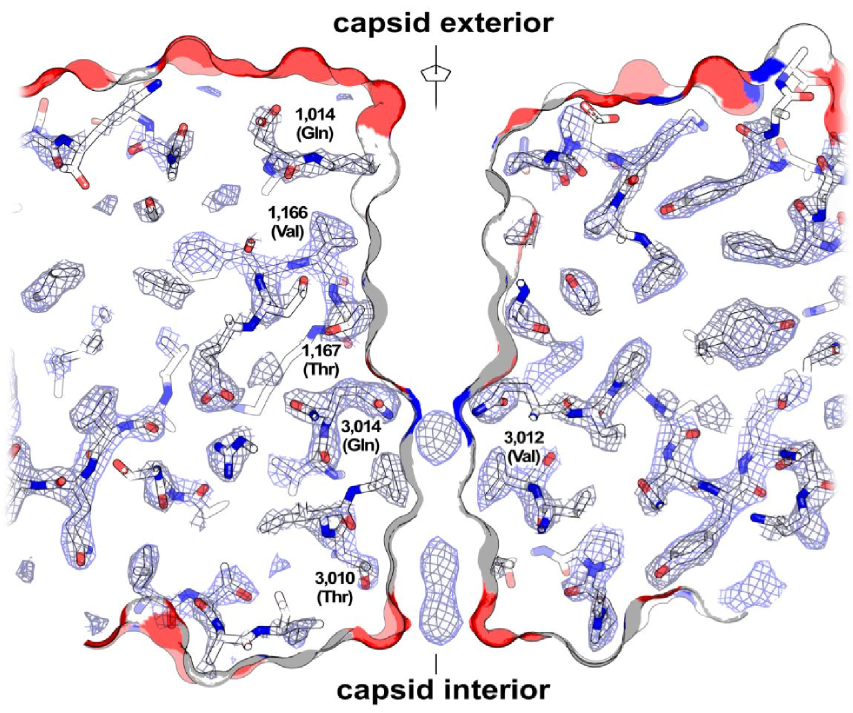
\includegraphics[height=6.5cm,keepaspectratio]{Figure/TrV_edens.png}};
    \draw<2>[red,ultra thick,rounded corners] (3.5,2.0) rectangle (4.5,3.0);
\end{tikzpicture} \\
\centering Mapa de densidad electrónica de TrV \\(Material Suplementario \textit{G. Squires et al 2013}).
\end{frame}

\subsection{Potencial de Fuerza Media}
\begin{frame}[t]{Perfil de Energía Libre en el poro de TrV}
La energía libre viene dada por la expresión:\\
\begin{minipage}{0.4\textwidth}
\begin{equation*}
A = - k_B T \ln Q
\end{equation*}
\end{minipage}
\onslide<2->{
\begin{minipage}{0.4\textwidth}
\begin{equation*}
A = k_B T \ln \left(\iint d\bm{p}^N d\bm{r}^N
\tikzmarkin<3->[set fill color=red!10, set border color=red]{pmf1}(0,-0.2)(0,0.6)
e^{\frac{E(\bm{p}^N,\bm{r}^N)}{k_B T}}
\tikzmarkend{pmf1}
\rho(\bm{p}^N,\bm{r}^N) \right)
\end{equation*}
\end{minipage}
}
\vspace{0.2cm}

\begin{columns}
\column{0.5\textwidth}
\onslide<4->{
\centering
\large
\tikzmarkin<4->[set fill color=green!10, set border color=green]{pmf2}(1,-0.5)(0,0.5)
{Potencial de Fuerza Media\\ o\\ \textbf{PMF}\\
$+$\\
Umbrella Sampling}
\tikzmarkend{pmf2}\\
}
\vspace{1cm}
\onslide<6->{
\centering
\large
\tikzmarkin<6->[set fill color=blue!10, set border color=blue]{pmf3}(1.2,-0.2)(0,0.5)
{Weighted Histogram\\ Analysis Method\\o\\\textbf{WHAM}}
\tikzmarkend{pmf3}
}
\column{0.5\textwidth}
\onslide<5->{
\begin{figure}[ht]
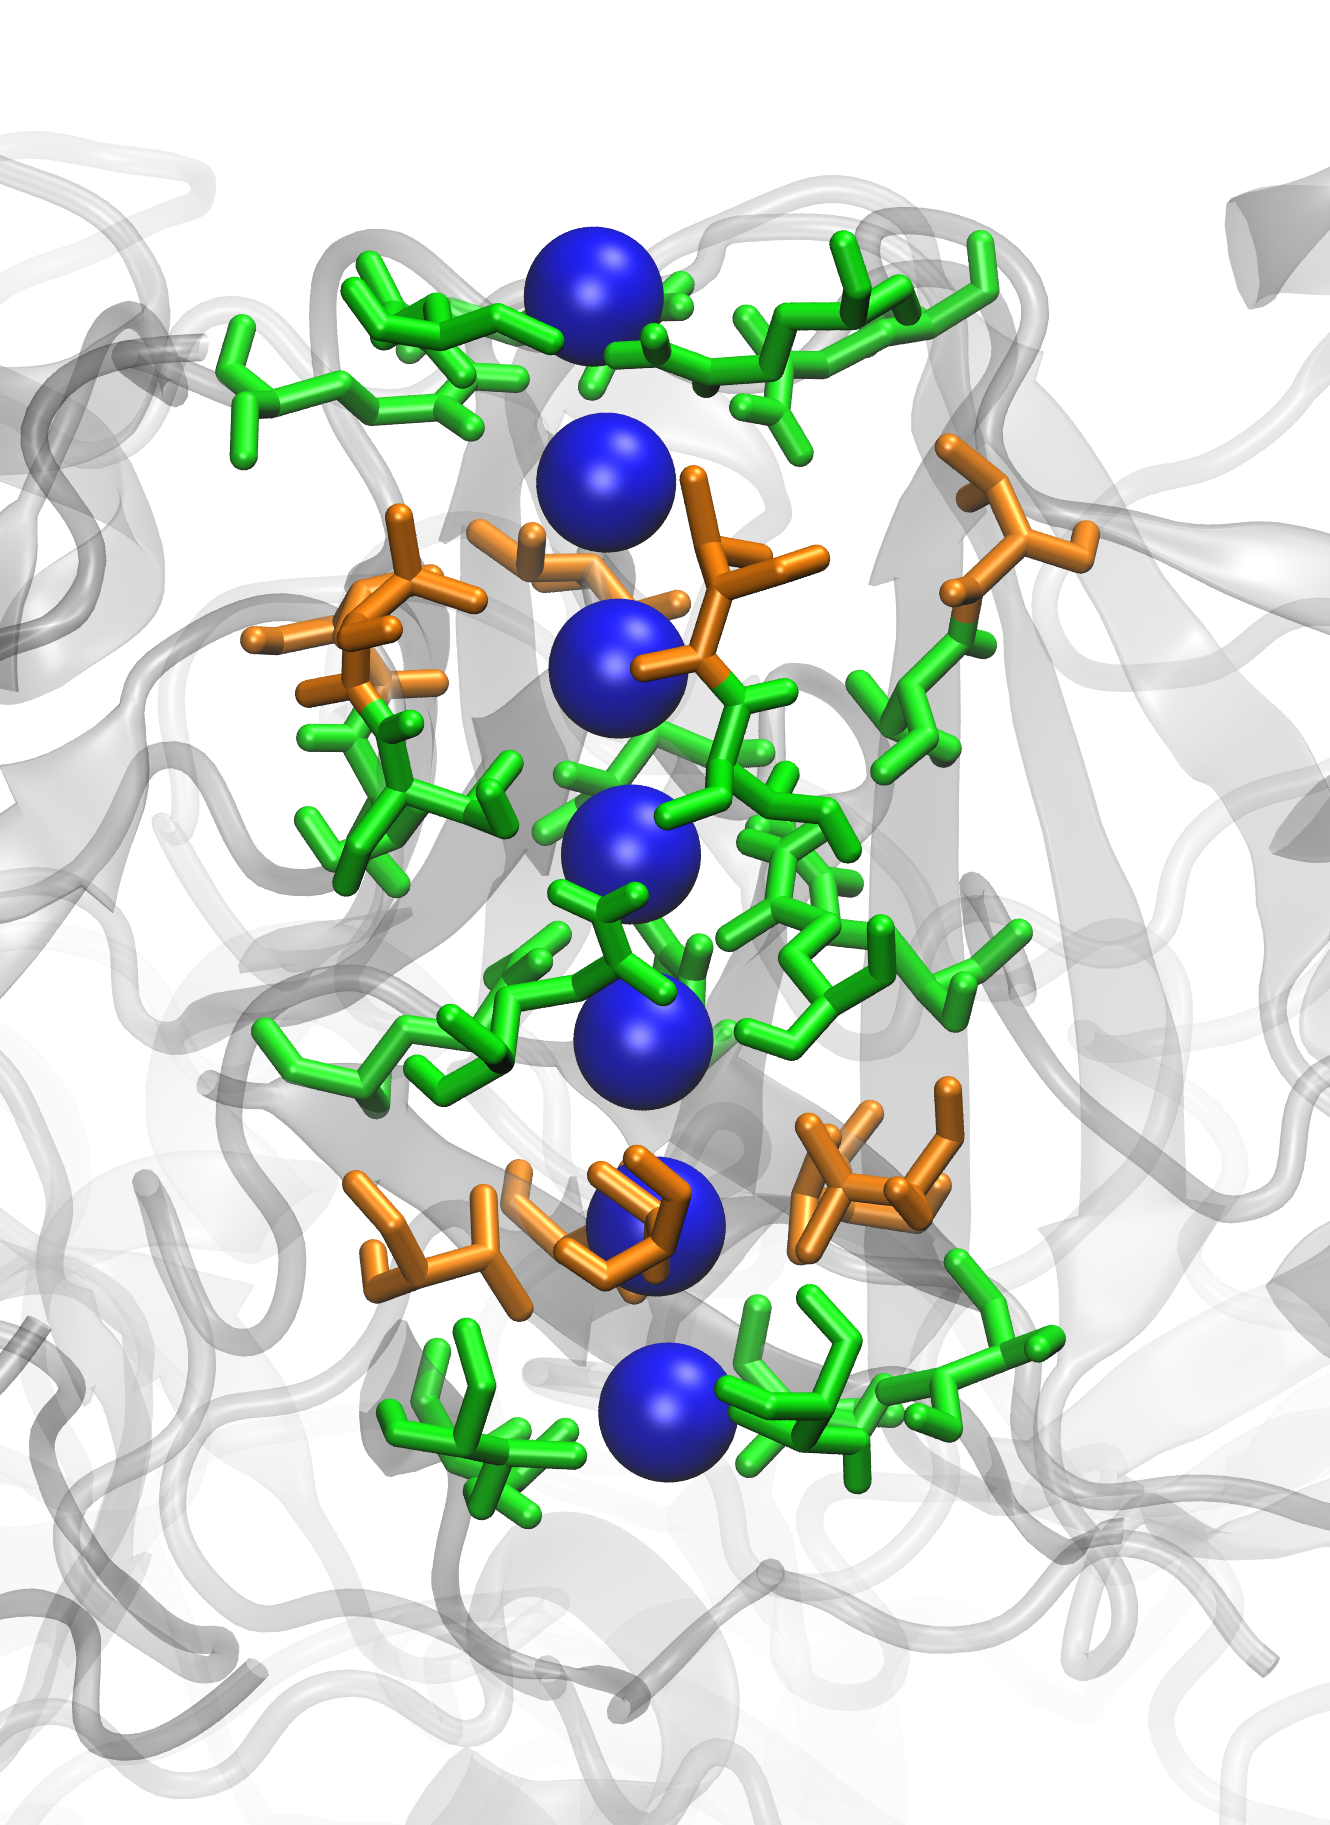
\includegraphics[width=0.6\textwidth]{Figure/TrV_pmf.png}
\end{figure}
}
\end{columns}
\end{frame}

\subsection{Perfil de Energía Libre en el poro de TrV}
\begin{frame}{Perfil de Energía Libre en el poro de TrV}
\begin{figure}[ht]
  \centering
  \only<1>{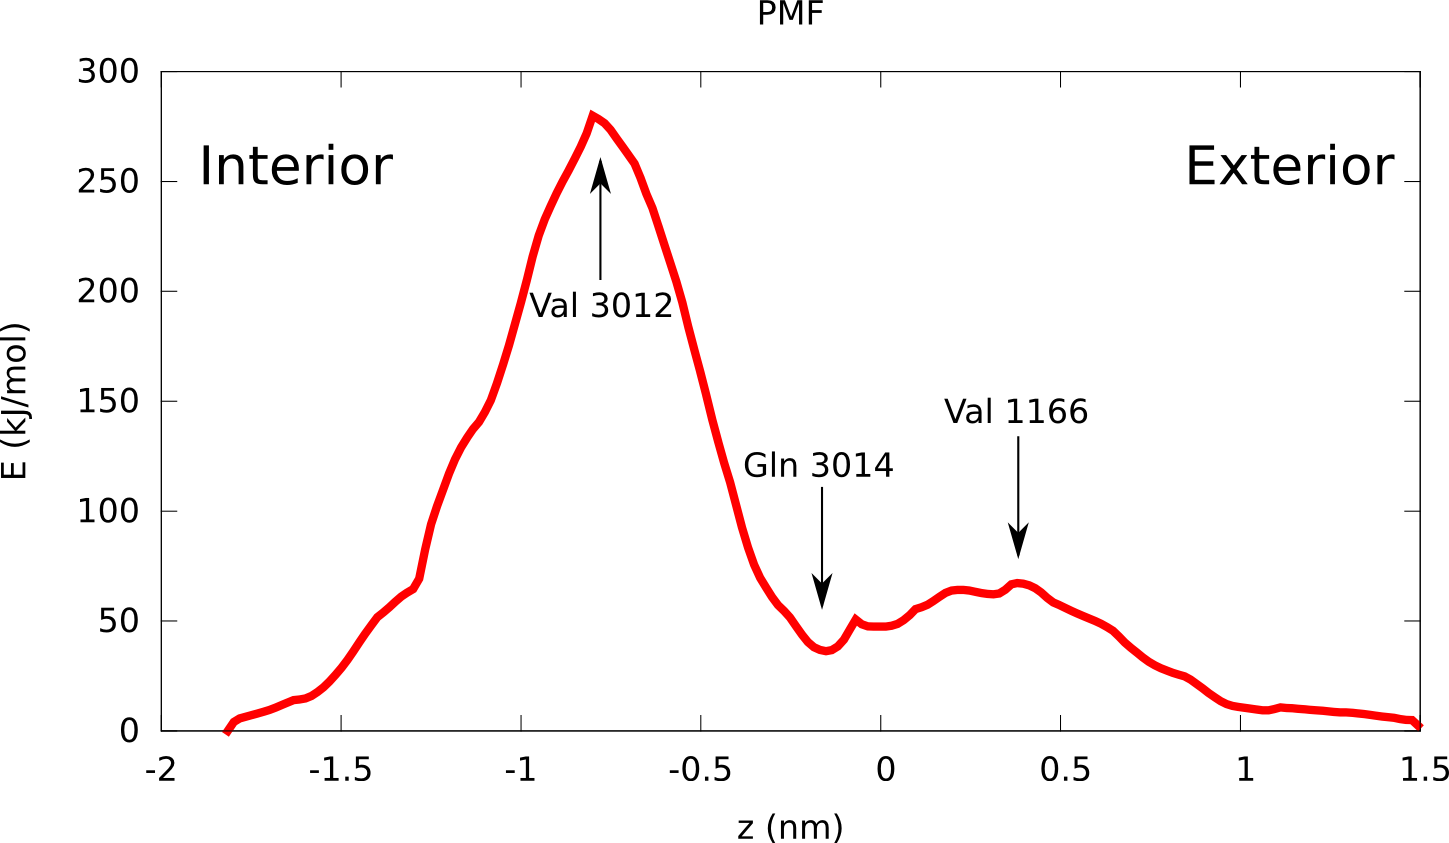
\includegraphics[width=0.7\textwidth]{Figure/profile1.png}}
  
    \begin{tikzpicture}
    \node[anchor=south west,inner sep=0] at (0,0)
    {\only<2-5>{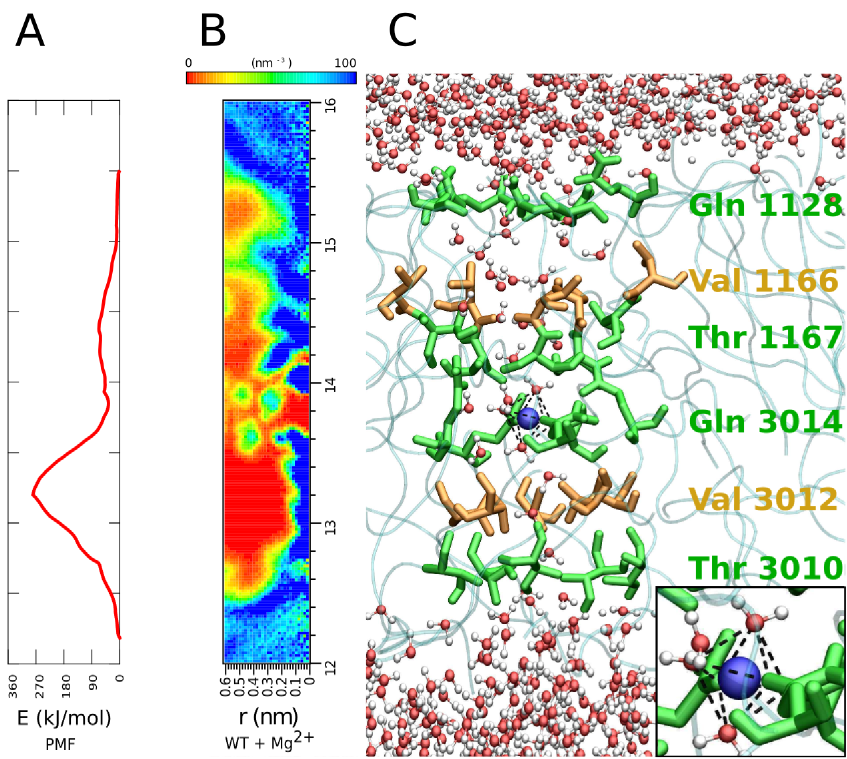
\includegraphics[height=6.3cm,keepaspectratio]{Figure/TrV_Mg_Dens.png}}};
    \draw<3,5>[violet,ultra thick,rounded corners] (0.0,2.6) rectangle (7.0,3.0);
    \draw<3,5>[violet,ultra thick,rounded corners] (0.0,2.0) rectangle (7.0,2.4);
    \end{tikzpicture} \\
  
  \caption*{(A) Energía Libre de Gibbs del Mg$^{2+}$ en función de la coordenada de reacción. (B) Mapa de densidad de moléculas de agua (C) Vista lateral del poro de TrV.}
\end{figure}

\begin{textblock*}{6cm}(0.5\textwidth,0.6\textheight)
\only<4>{
\begin{figure}
    \centering
    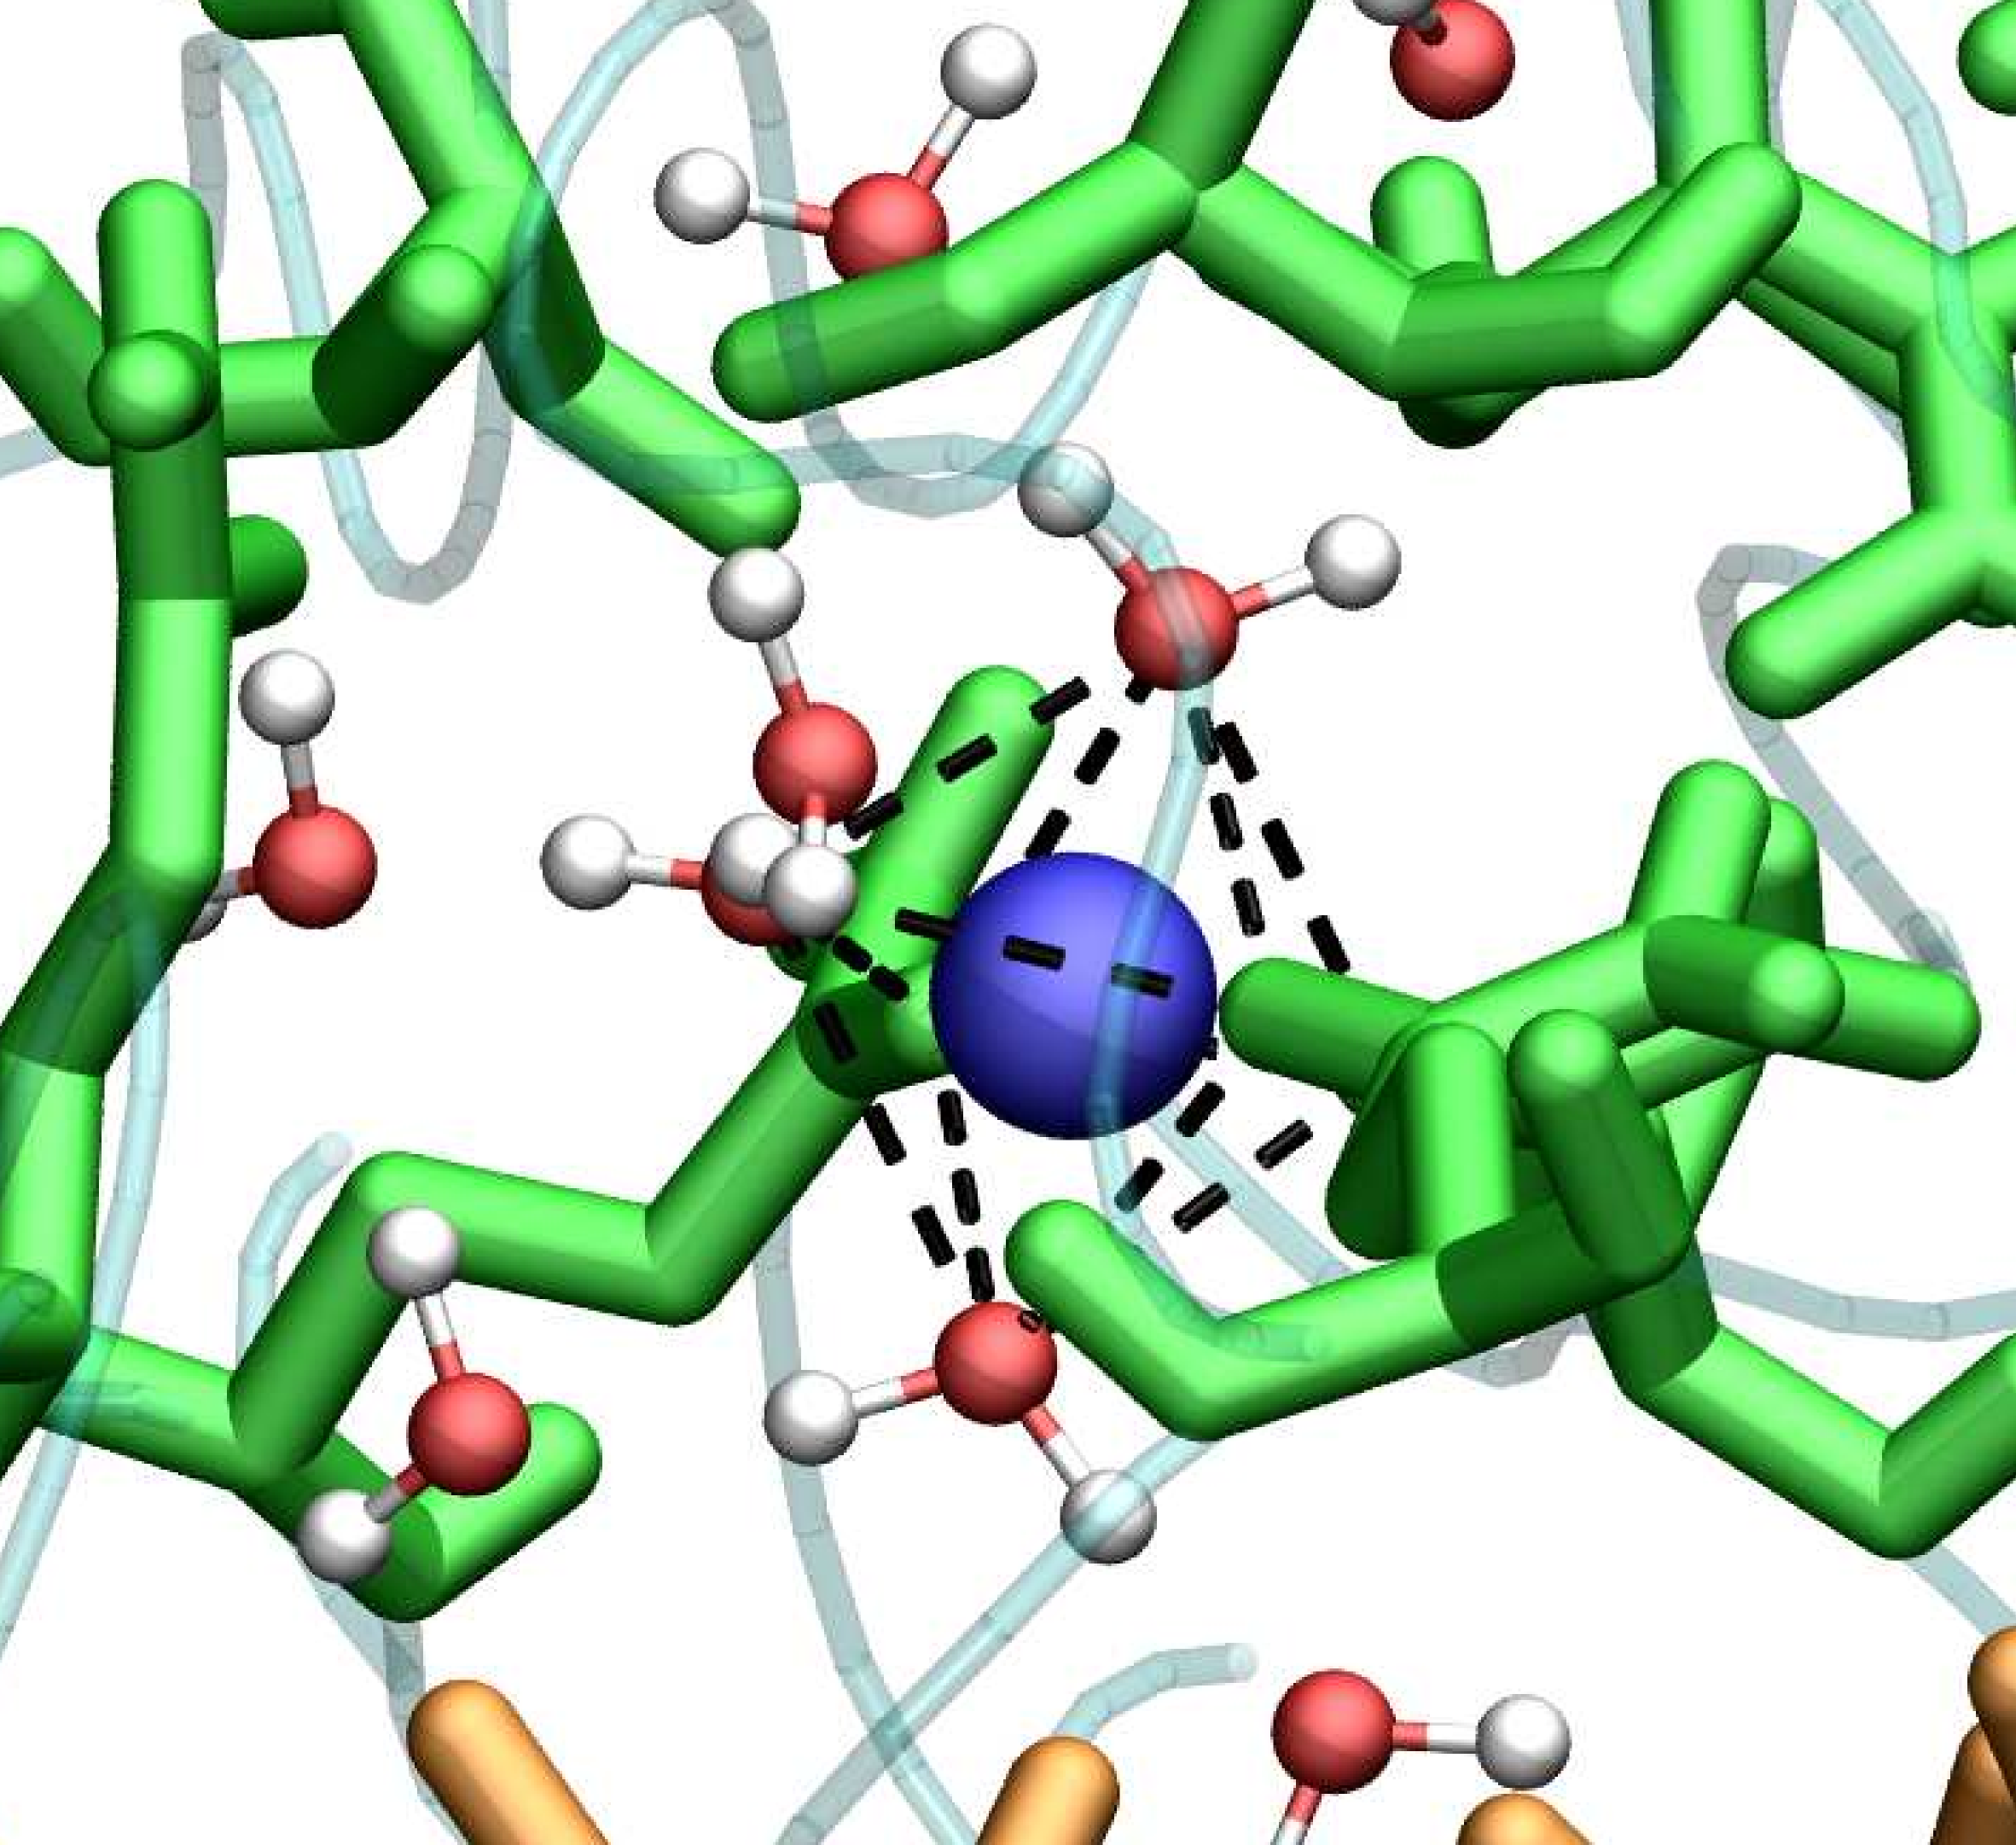
\includegraphics[width=0.7\textwidth]{Figure/mg_sol.png}
\end{figure}}
\end{textblock*}

\end{frame}

\subsection{Conclusión II}
\begin{frame}{Conclusión II}
\begin{itemize}
    \item La presencia de un ion \alert{Mg$^{2+}$} en el poro a nivel de las Glutaminas 3014 logra la \alert{completa hidratación del poro}.\vfill
    \item El perfil de energía libre nos indica que el \alert{ingreso de los iones} ocurre \alert{desde el exterior} de la cápside ya que de lo contrario, lo iones deberían atravesar una barrera energética mayor.\vfill
    \item La ausencia de un flujo de moléculas de aguas en conjunto con la cadena continua de aguas podrían indicar la existencia de una posible \alert{cadena transportadora de protones}.
\end{itemize}
\end{frame}

%
% Otros Virus
%

\section{Otros Virus}
\subsection{Puerta Hidrofóbica en otros Virus}
\begin{frame}{Puerta Hidrofóbica en otros Virus}
\hspace{-0.7cm}
\begin{minipage}[t]{0.4\textwidth}
\begin{itemize}
    \item<1-> Picornavirus.
    \begin{itemize}
    \item<1-> Human Rhinovirus 16.
    \item<2-> Poliovirus.
    \item<3-> Hepatitis A Virus.
    \end{itemize}
    \item<4-> Dicistrovirus.
    \begin{itemize}
    \item<4-> Cricket Paralysis Virus.
    \item<4-> Triatoma Virus.
    \end{itemize}
    \item<5-> Secovirus.
    \begin{itemize}
    \item<5-> Bean Pod Mottle Virus.
    \item<6-> Tobacco Ringspot Virus.
    \end{itemize}
\end{itemize}
\end{minipage}
\begin{minipage}[t]{0.6\textwidth}
\only<1>{
\begin{figure}[ht]
  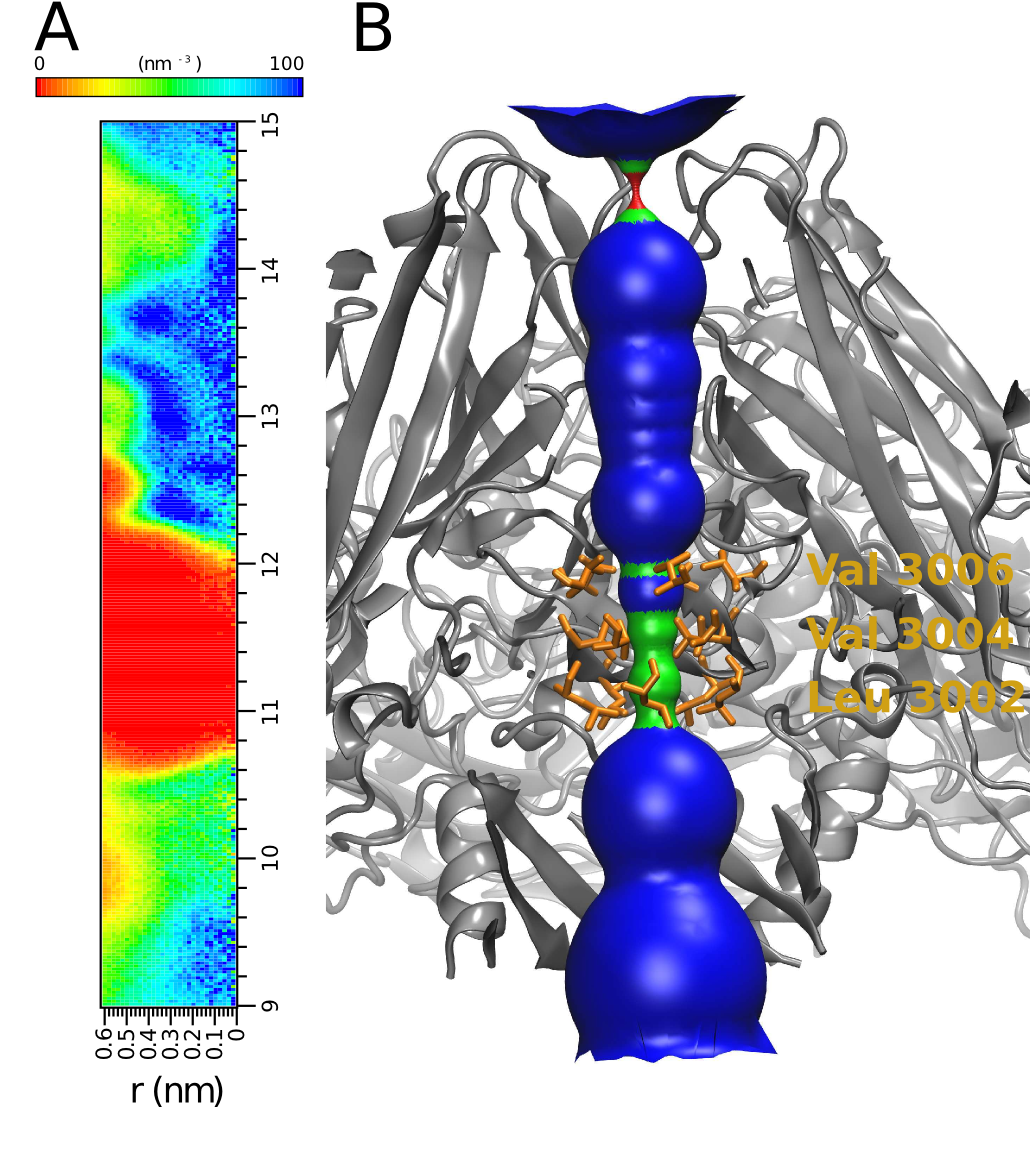
\includegraphics[height=7cm,keepaspectratio]{Figure/HRV16_Densmap.png}
\end{figure}
}
\only<2>{
\begin{figure}[ht]
  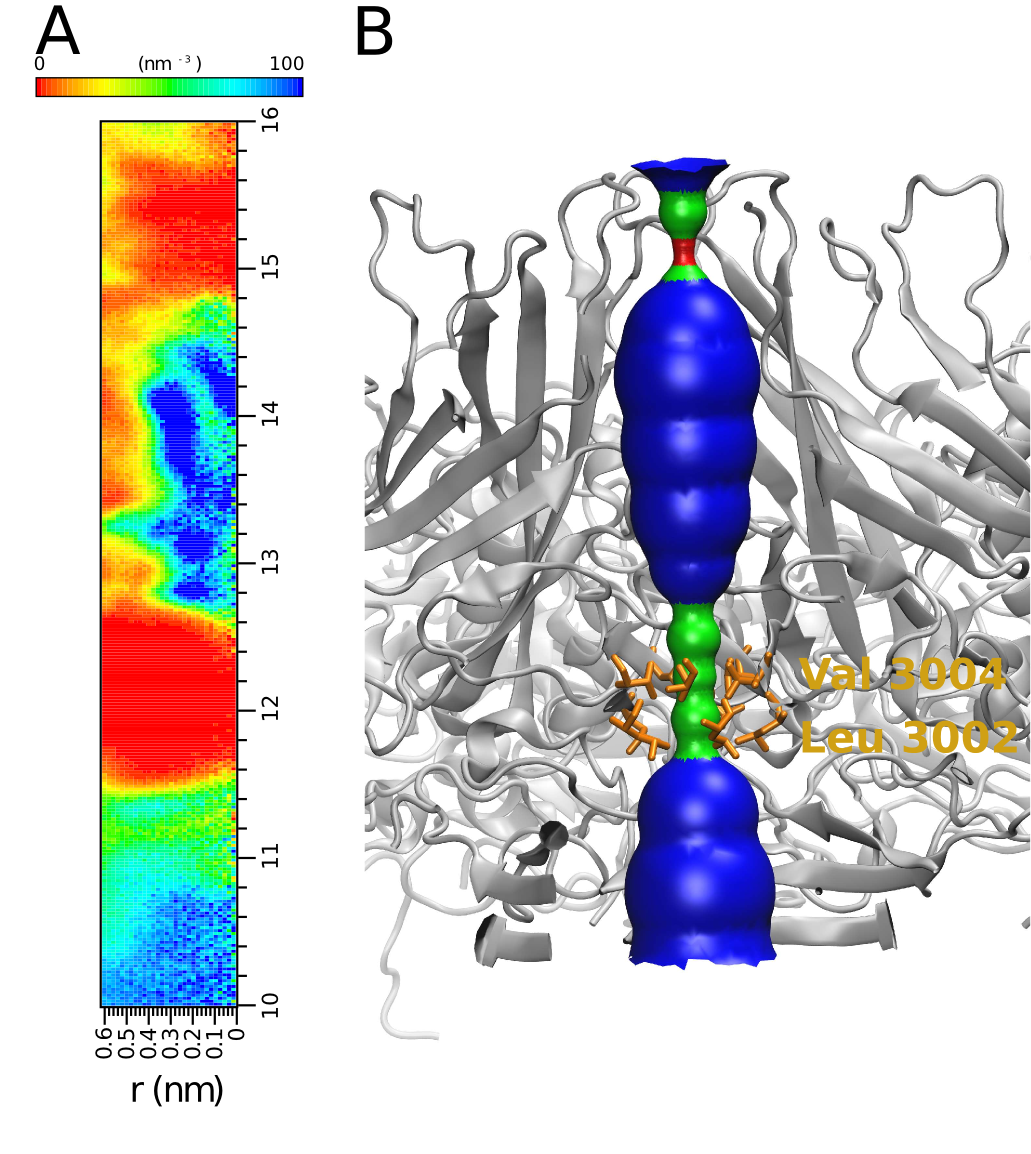
\includegraphics[height=7cm,keepaspectratio]{Figure/PoV_Densmap.png}
\end{figure}
}
\only<3>{
\begin{figure}[ht]
  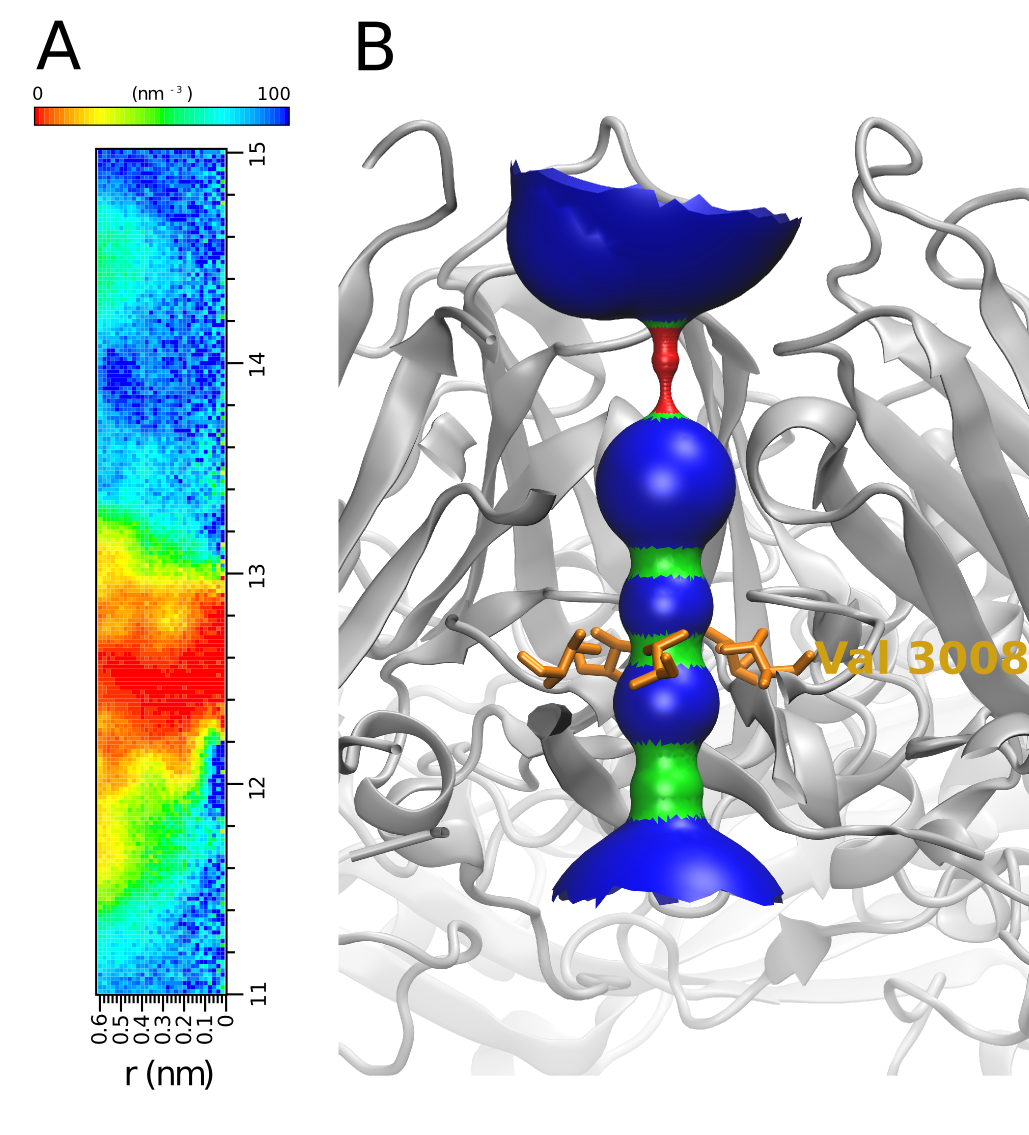
\includegraphics[height=7cm,keepaspectratio]{Figure/HAV_Densmap.png}
\end{figure}
}
\only<4>{
\begin{figure}[ht]
  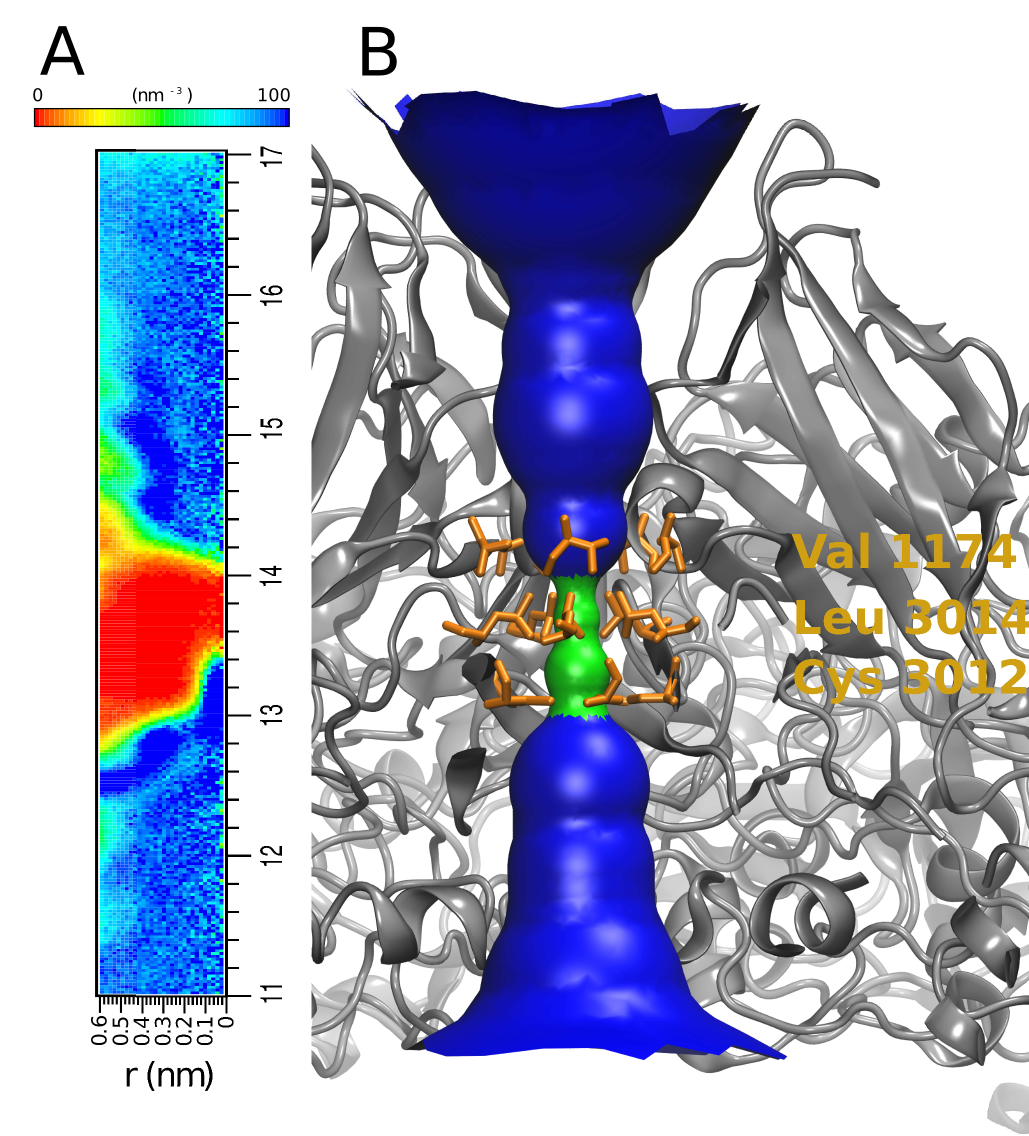
\includegraphics[height=7cm,keepaspectratio]{Figure/CrPV_Densmap.png}
\end{figure}
}
\only<5>{
\begin{figure}[ht]
  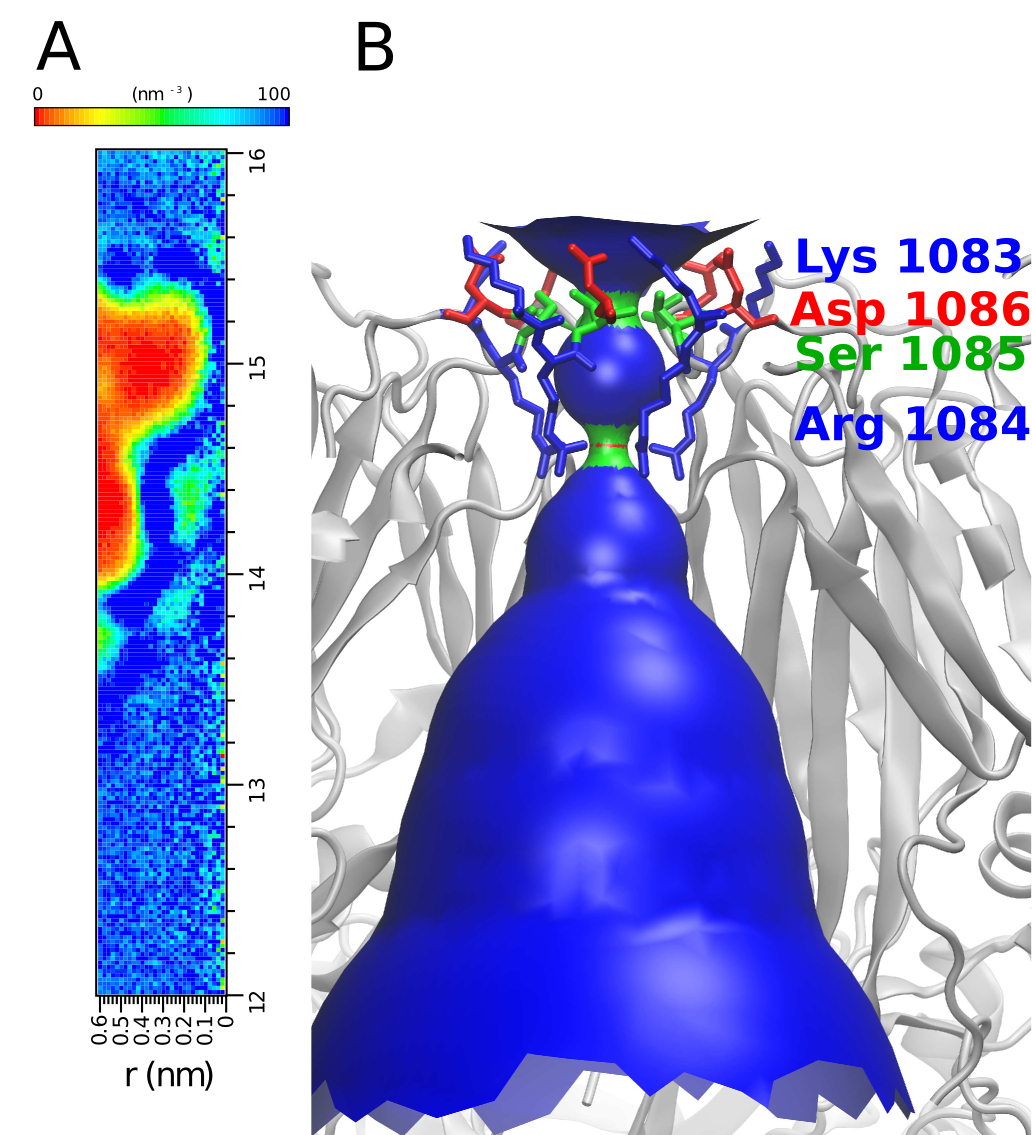
\includegraphics[height=7cm,keepaspectratio]{Figure/BPMV_Densmap.png}
\end{figure}
}
\only<6>{
\begin{figure}[ht]
  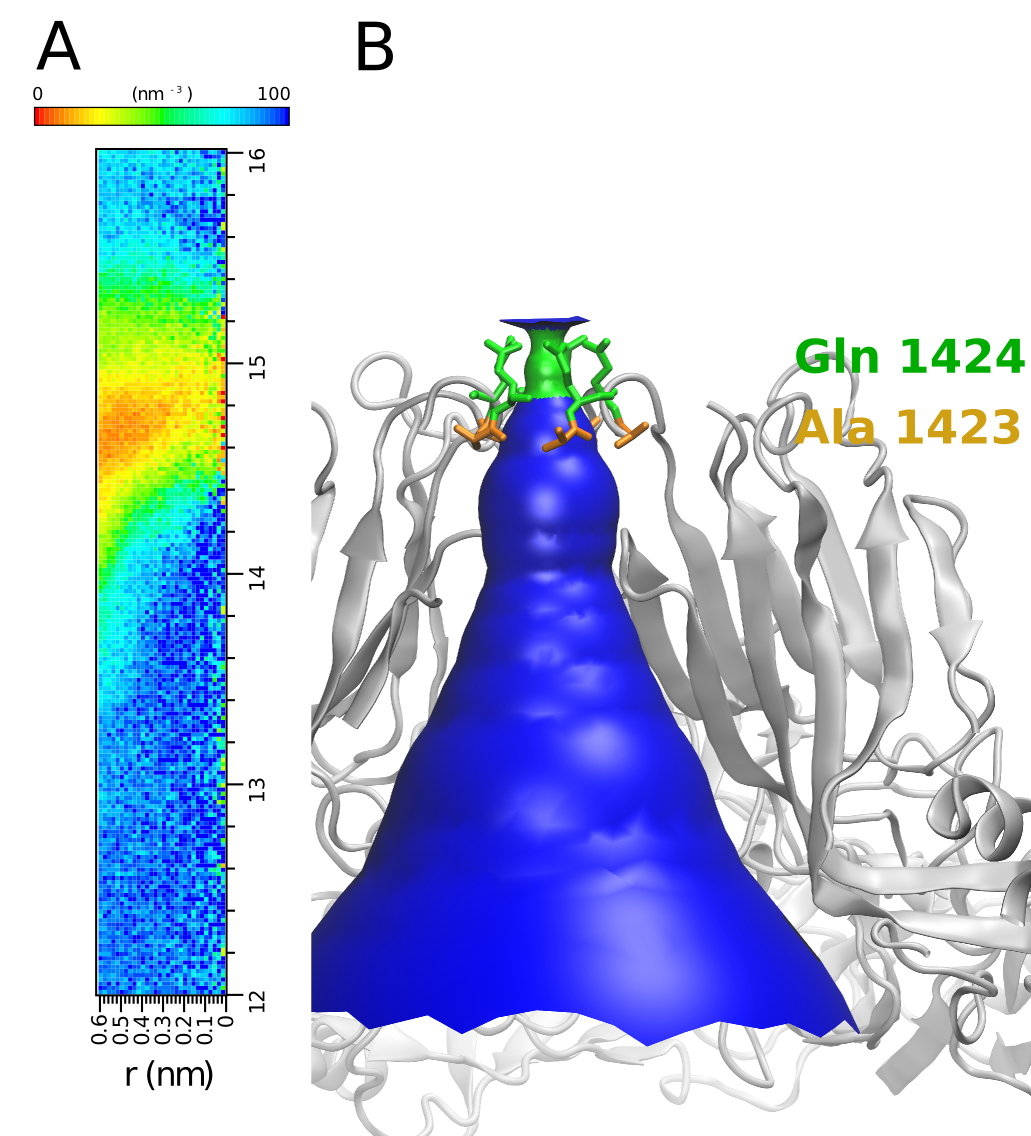
\includegraphics[height=7cm,keepaspectratio]{Figure/TRsV_Densmap.png}
\end{figure}
}
\end{minipage}
\end{frame}

\subsection{Conclusión III}
\begin{frame}{Conclusión III}
\begin{itemize}
    \item Los virus pertenecientes al orden \textit{Picornavirales} que infectan a animales (\alert{\textit{Picornavirus}}) e insectos (\alert{\textit{Dicistrovirus}}), \alert{presentan una puerta hidrofóbica} en el poro presente en el eje quíntuple.\vfill
    \item Los virus de la familia \alert{\textit{Secovirus}}, que infectan a vegetales, \alert{no presenta el mismo mecanismo de puerta hidrofóbica}.
\end{itemize}
\end{frame}

%
% Conclusión
%

\section{Conclusión}
\begin{frame}{Conclusión}
\begin{block}{¿Existe algún mecanismo de transporte en el eje quíntuple del Virus del Triatoma?}
\onslide<2->El Virus del Triatoma presenta un poro en su eje quíntuple que se encuentra cerrado (deshidratado) debido a una puerta hidrofóbica ubicada a la altura del anillo de aminoácidos formado por las Valinas 3012.
\end{block}
\onslide<3->\begin{block}{¿De qué manera regula su apertura?}
\onslide<4->La inserción de un ion Mg$^{2+}$ en el poro y su consecuente interacción con las Glutaminas 3014 ubicadas dentro del poro provocan la completa hidratación del poro. De esta manera, se logra la apertura del poro.
\end{block}
\onslide<5->\begin{block}{¿Qué tipo de moléculas son capaces de atravesarlo?}
\onslide<6->La formación de una cadena continua de moléculas de agua desde el exterior de la cápside hasta su interior podría indicar la existencia de un mecanismo de transporte de protones.
\end{block}
\end{frame}

\begin{frame}[t]{Palabras Finales}
\hspace{-0.8cm}
\begin{minipage}[t]{0.5\textwidth}
\centering
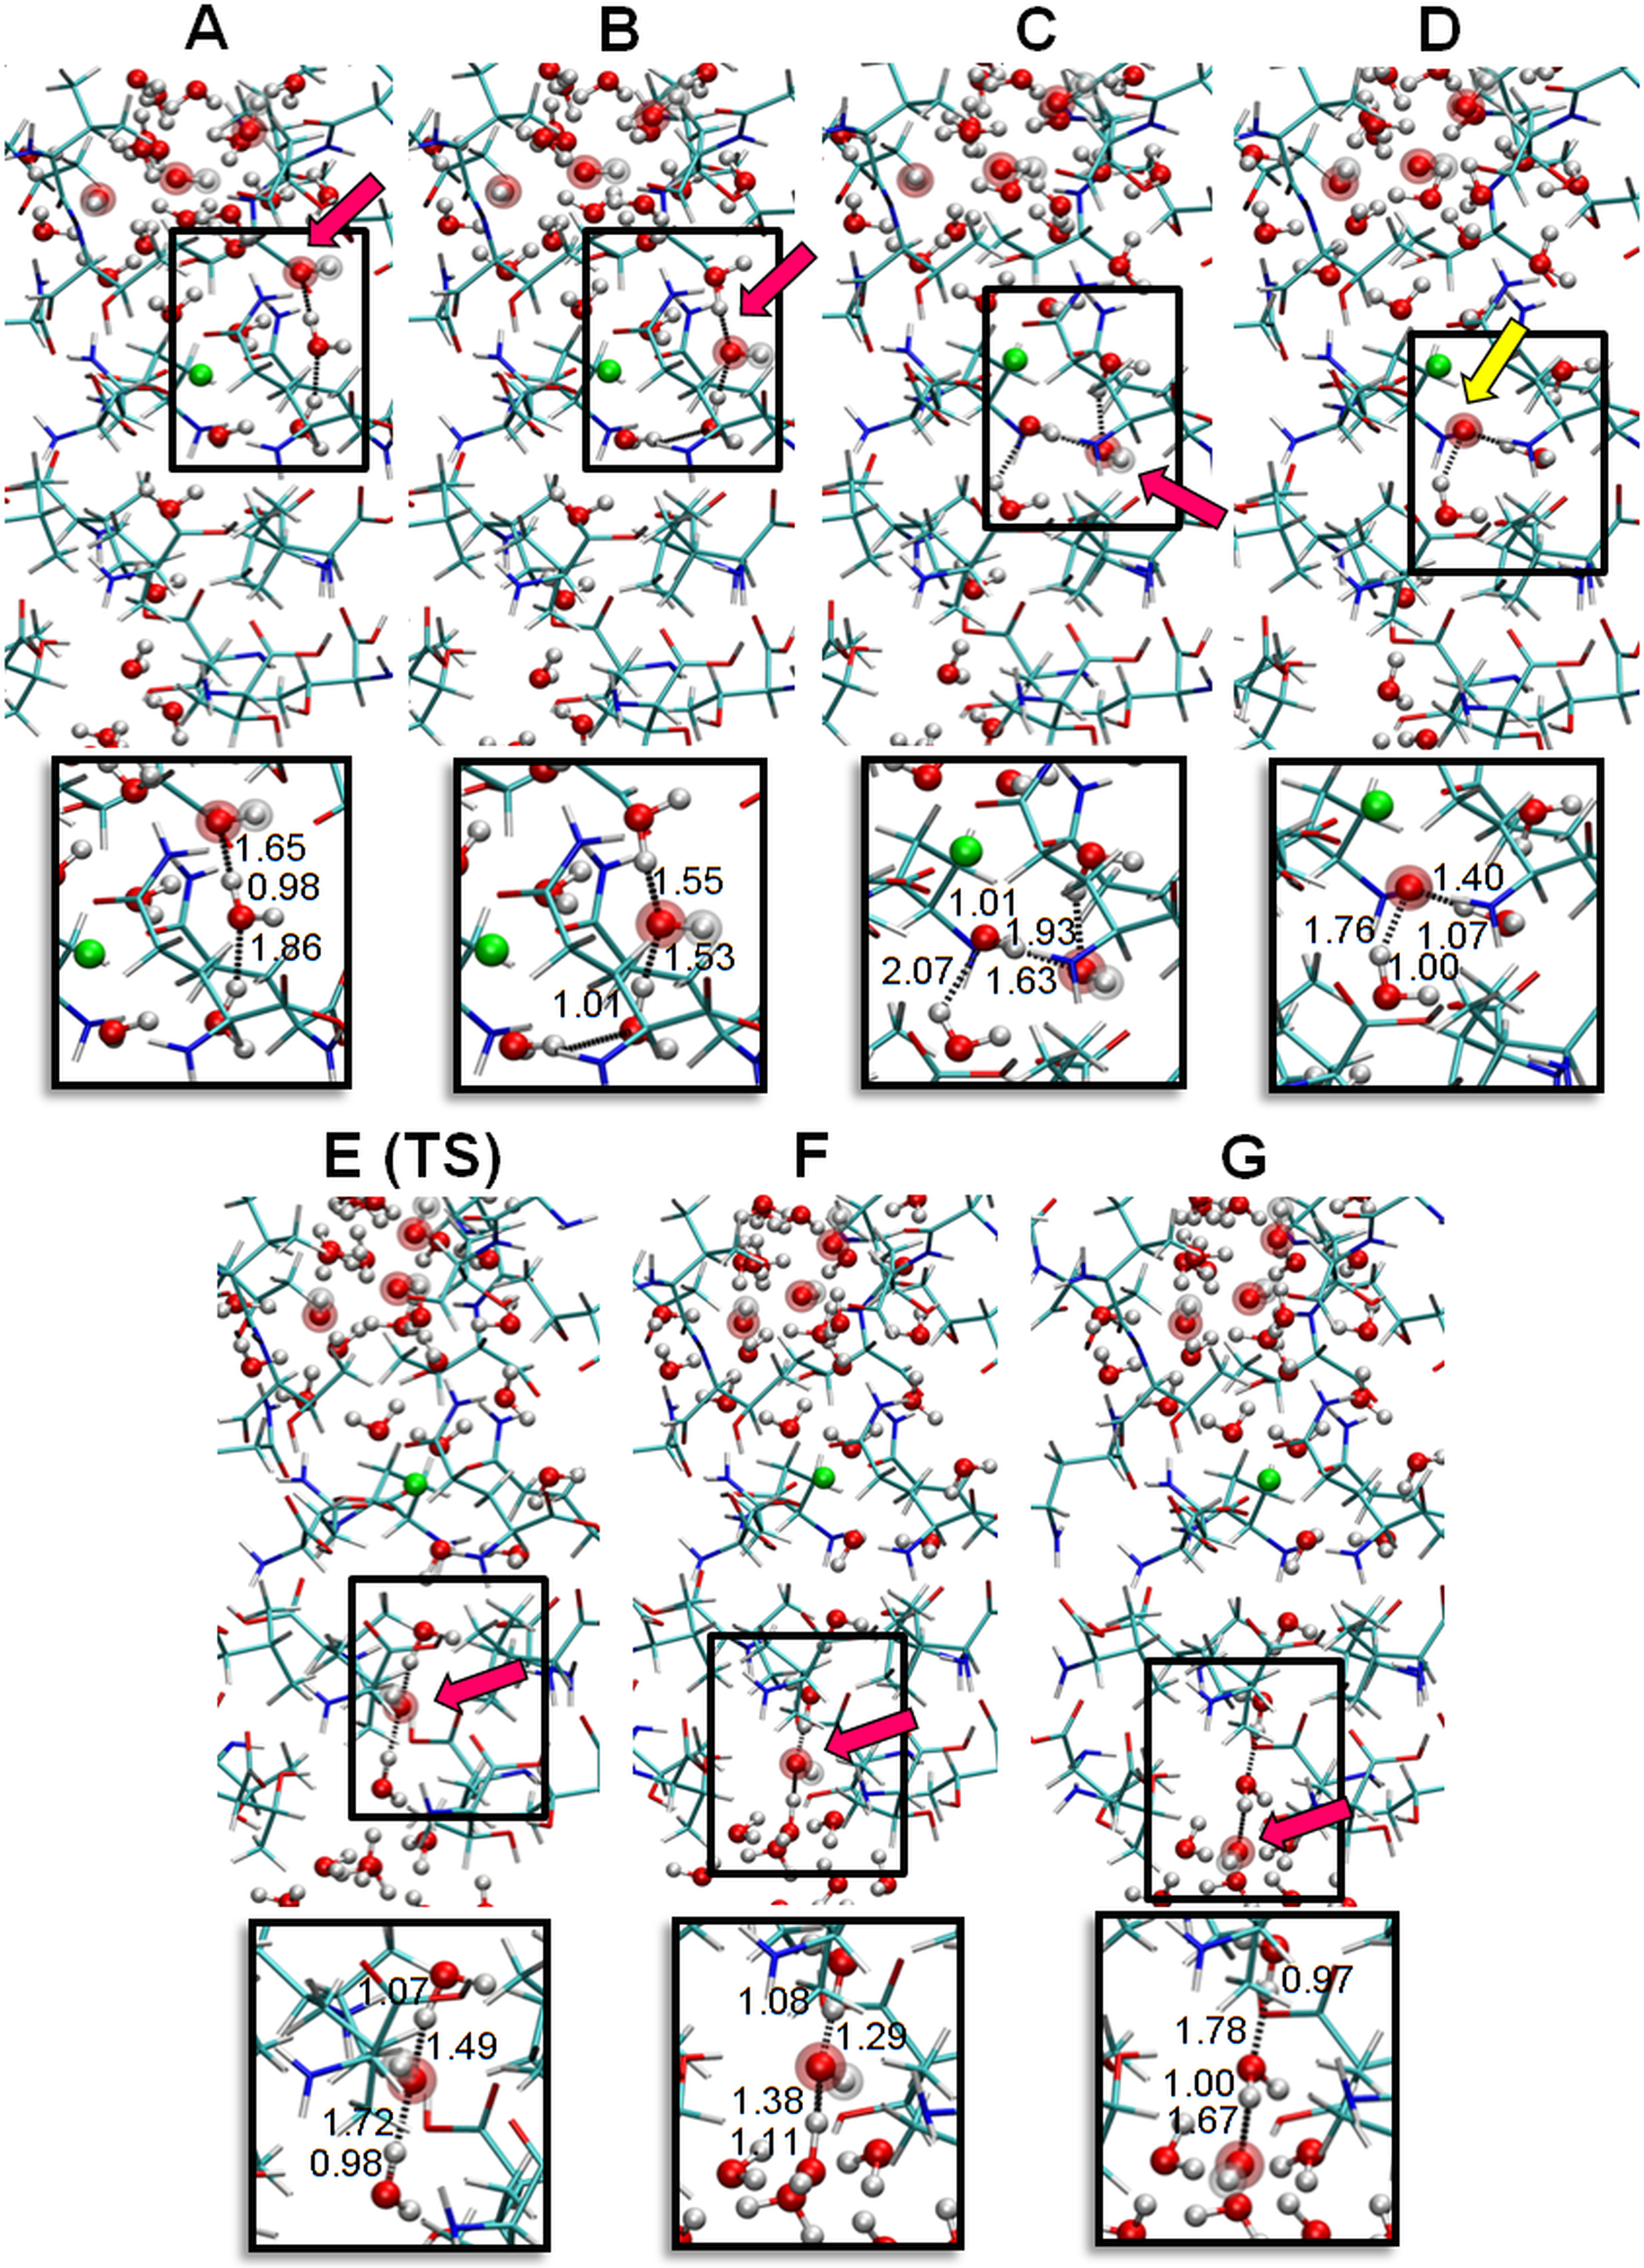
\includegraphics[height=7cm]{Figure/grothuss.png}
\end{minipage}
\begin{minipage}[t]{0.5\textwidth}
\centering
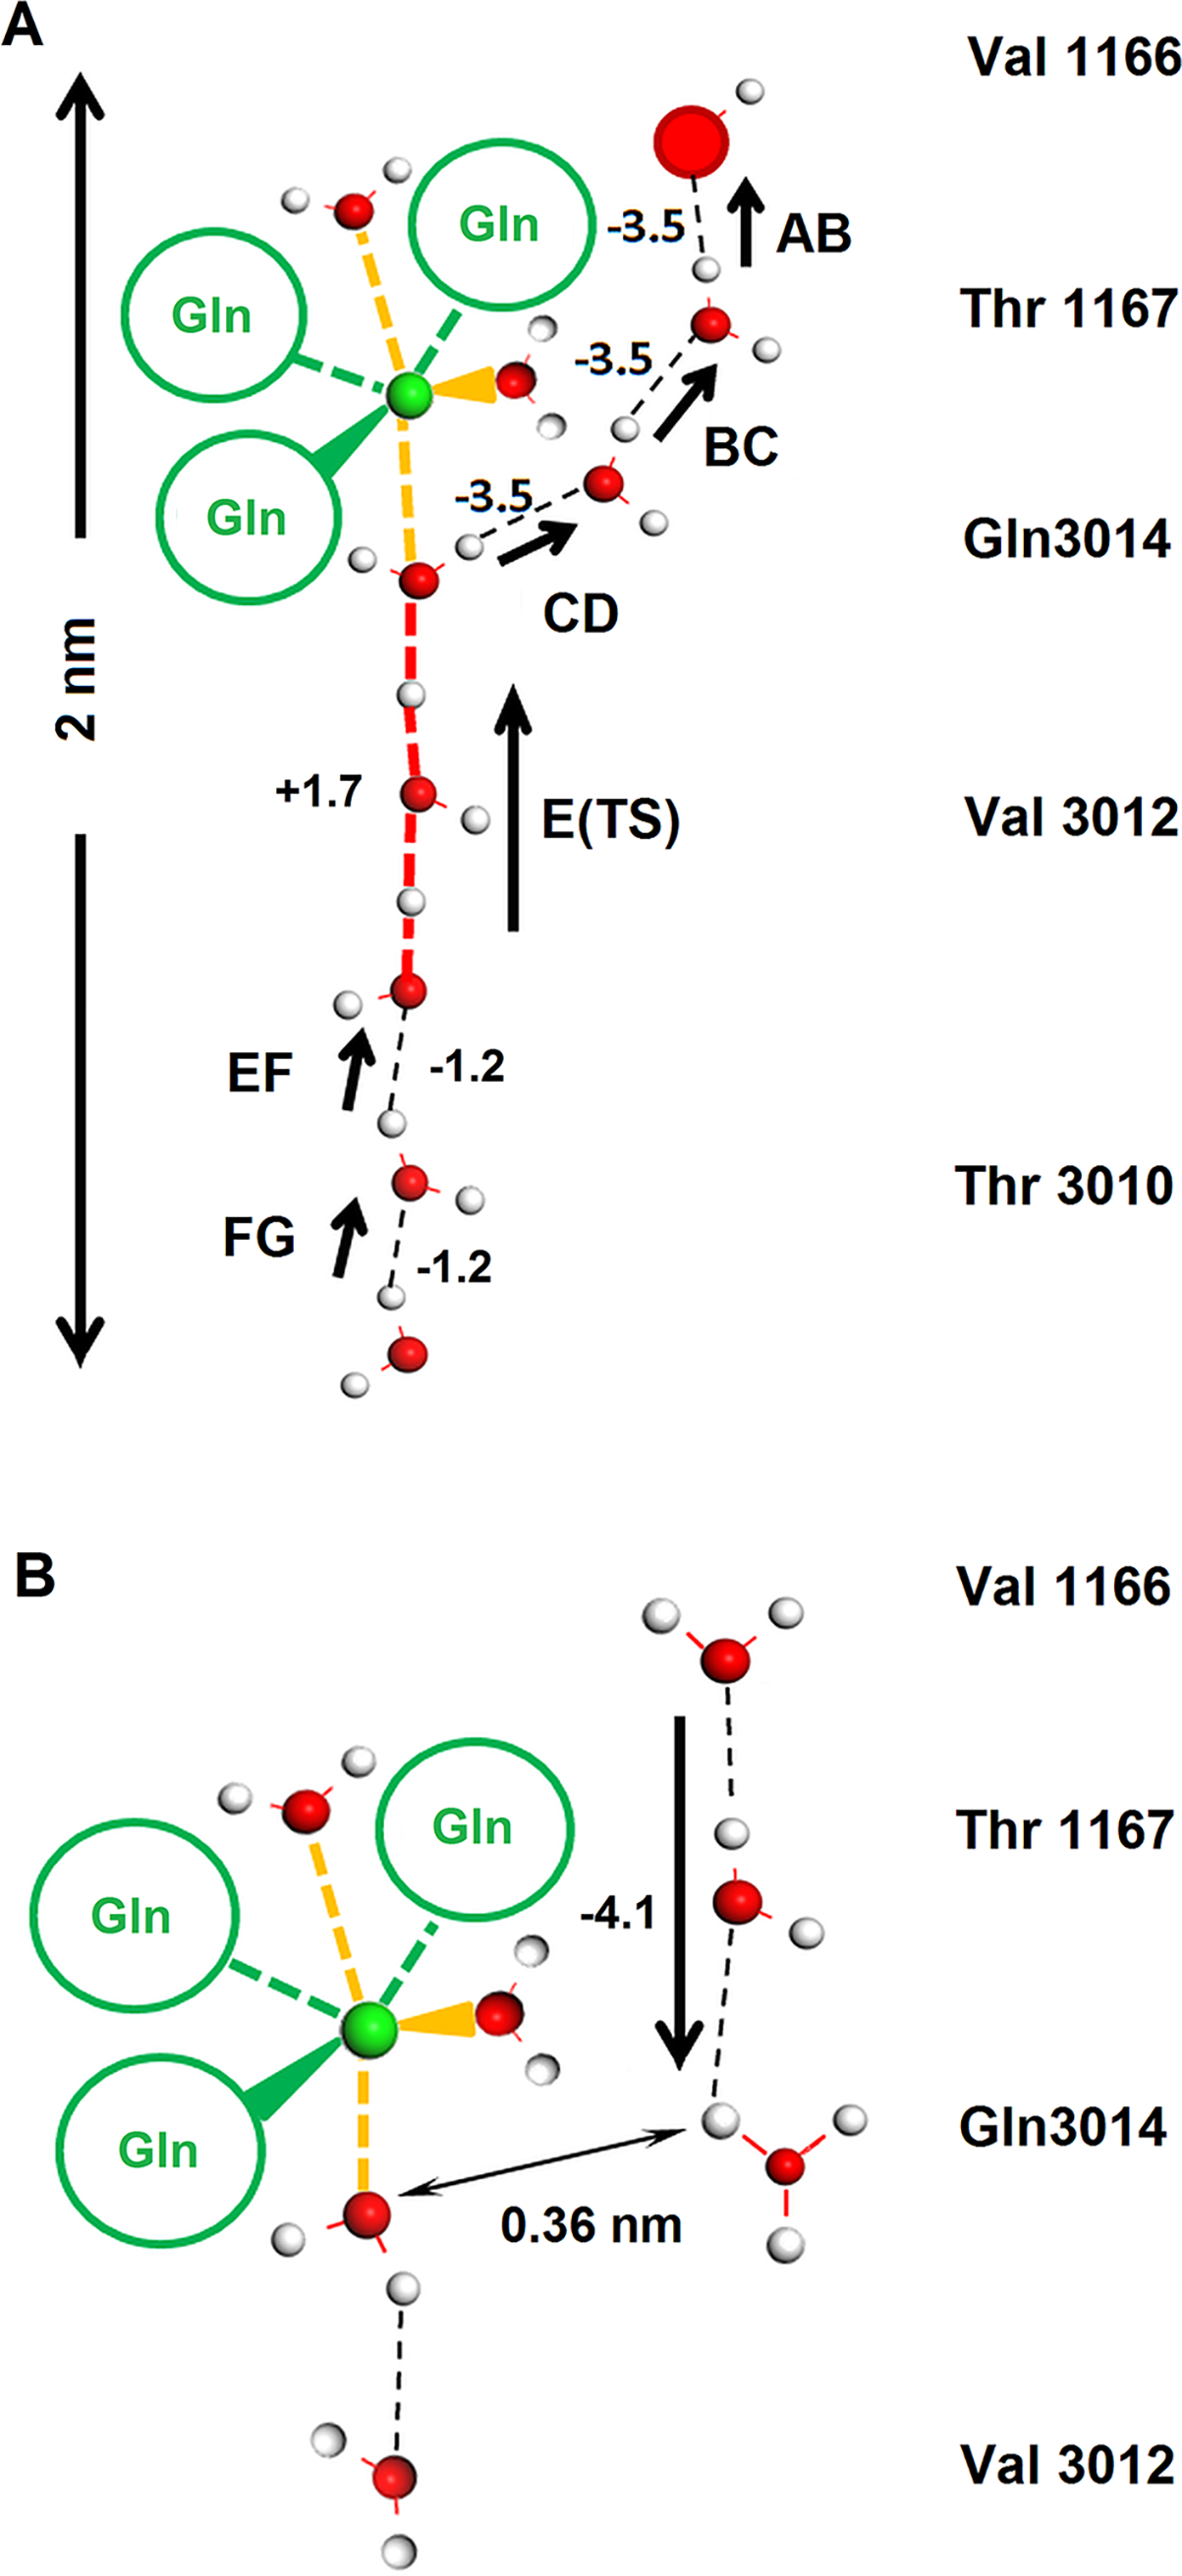
\includegraphics[height=7cm]{Figure/grothuss_2.png}
\onslide<2->\includegraphics[height=7cm]{Figure/paper.png}
\end{minipage}
\end{frame}

\begin{frame}
\centering
\begin{columns}
\begin{column}{0.2\textwidth}
\centering
\includegraphics[width=0.8\textwidth]{Figure/conclusion.png}
\end{column}
\begin{column}{0.6\textwidth}
\vfill
\centering
\Large En definitiva, los resultados expuestos en esta tesis son los que dan lugar a la posibilidad de explicar, por primera vez, el mecanismo de desensamblaje de una cápside viral.
\vfill
\end{column}
\begin{column}{0.2\textwidth}
\centering
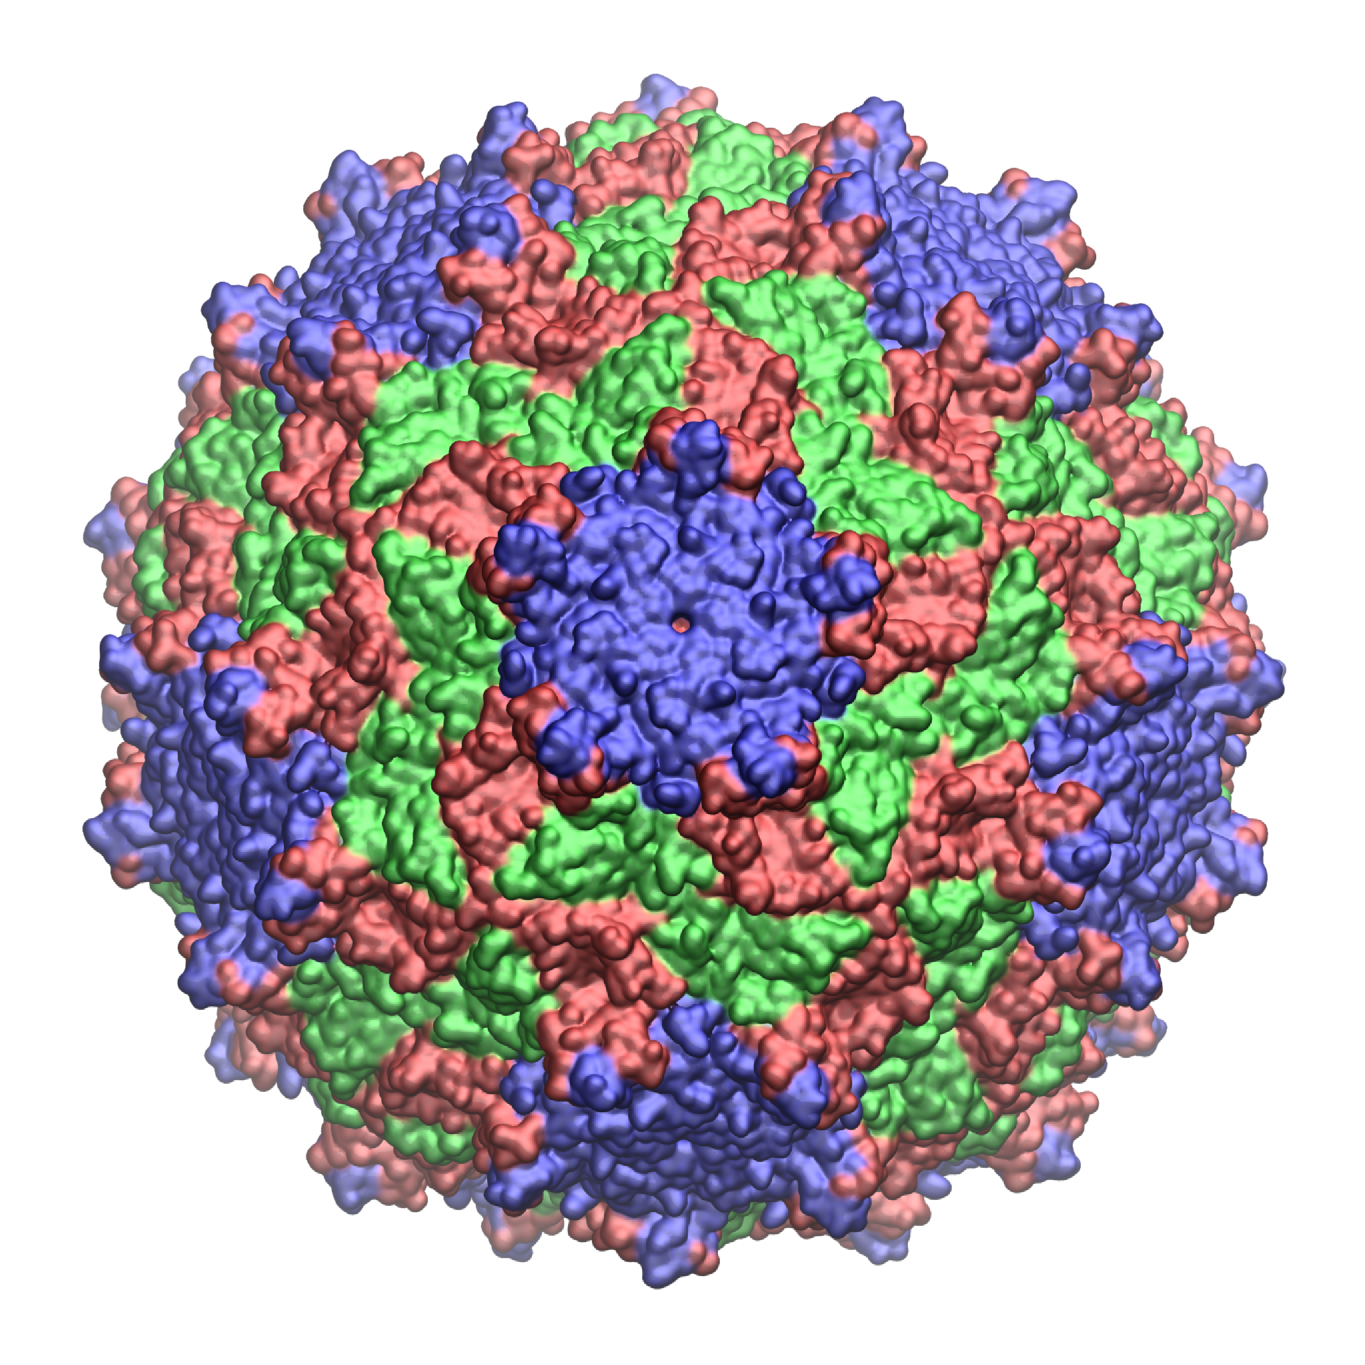
\includegraphics[width=0.8\textwidth]{Figure/TrV_Capsid_Ch4.png}\\
\vspace{3cm}
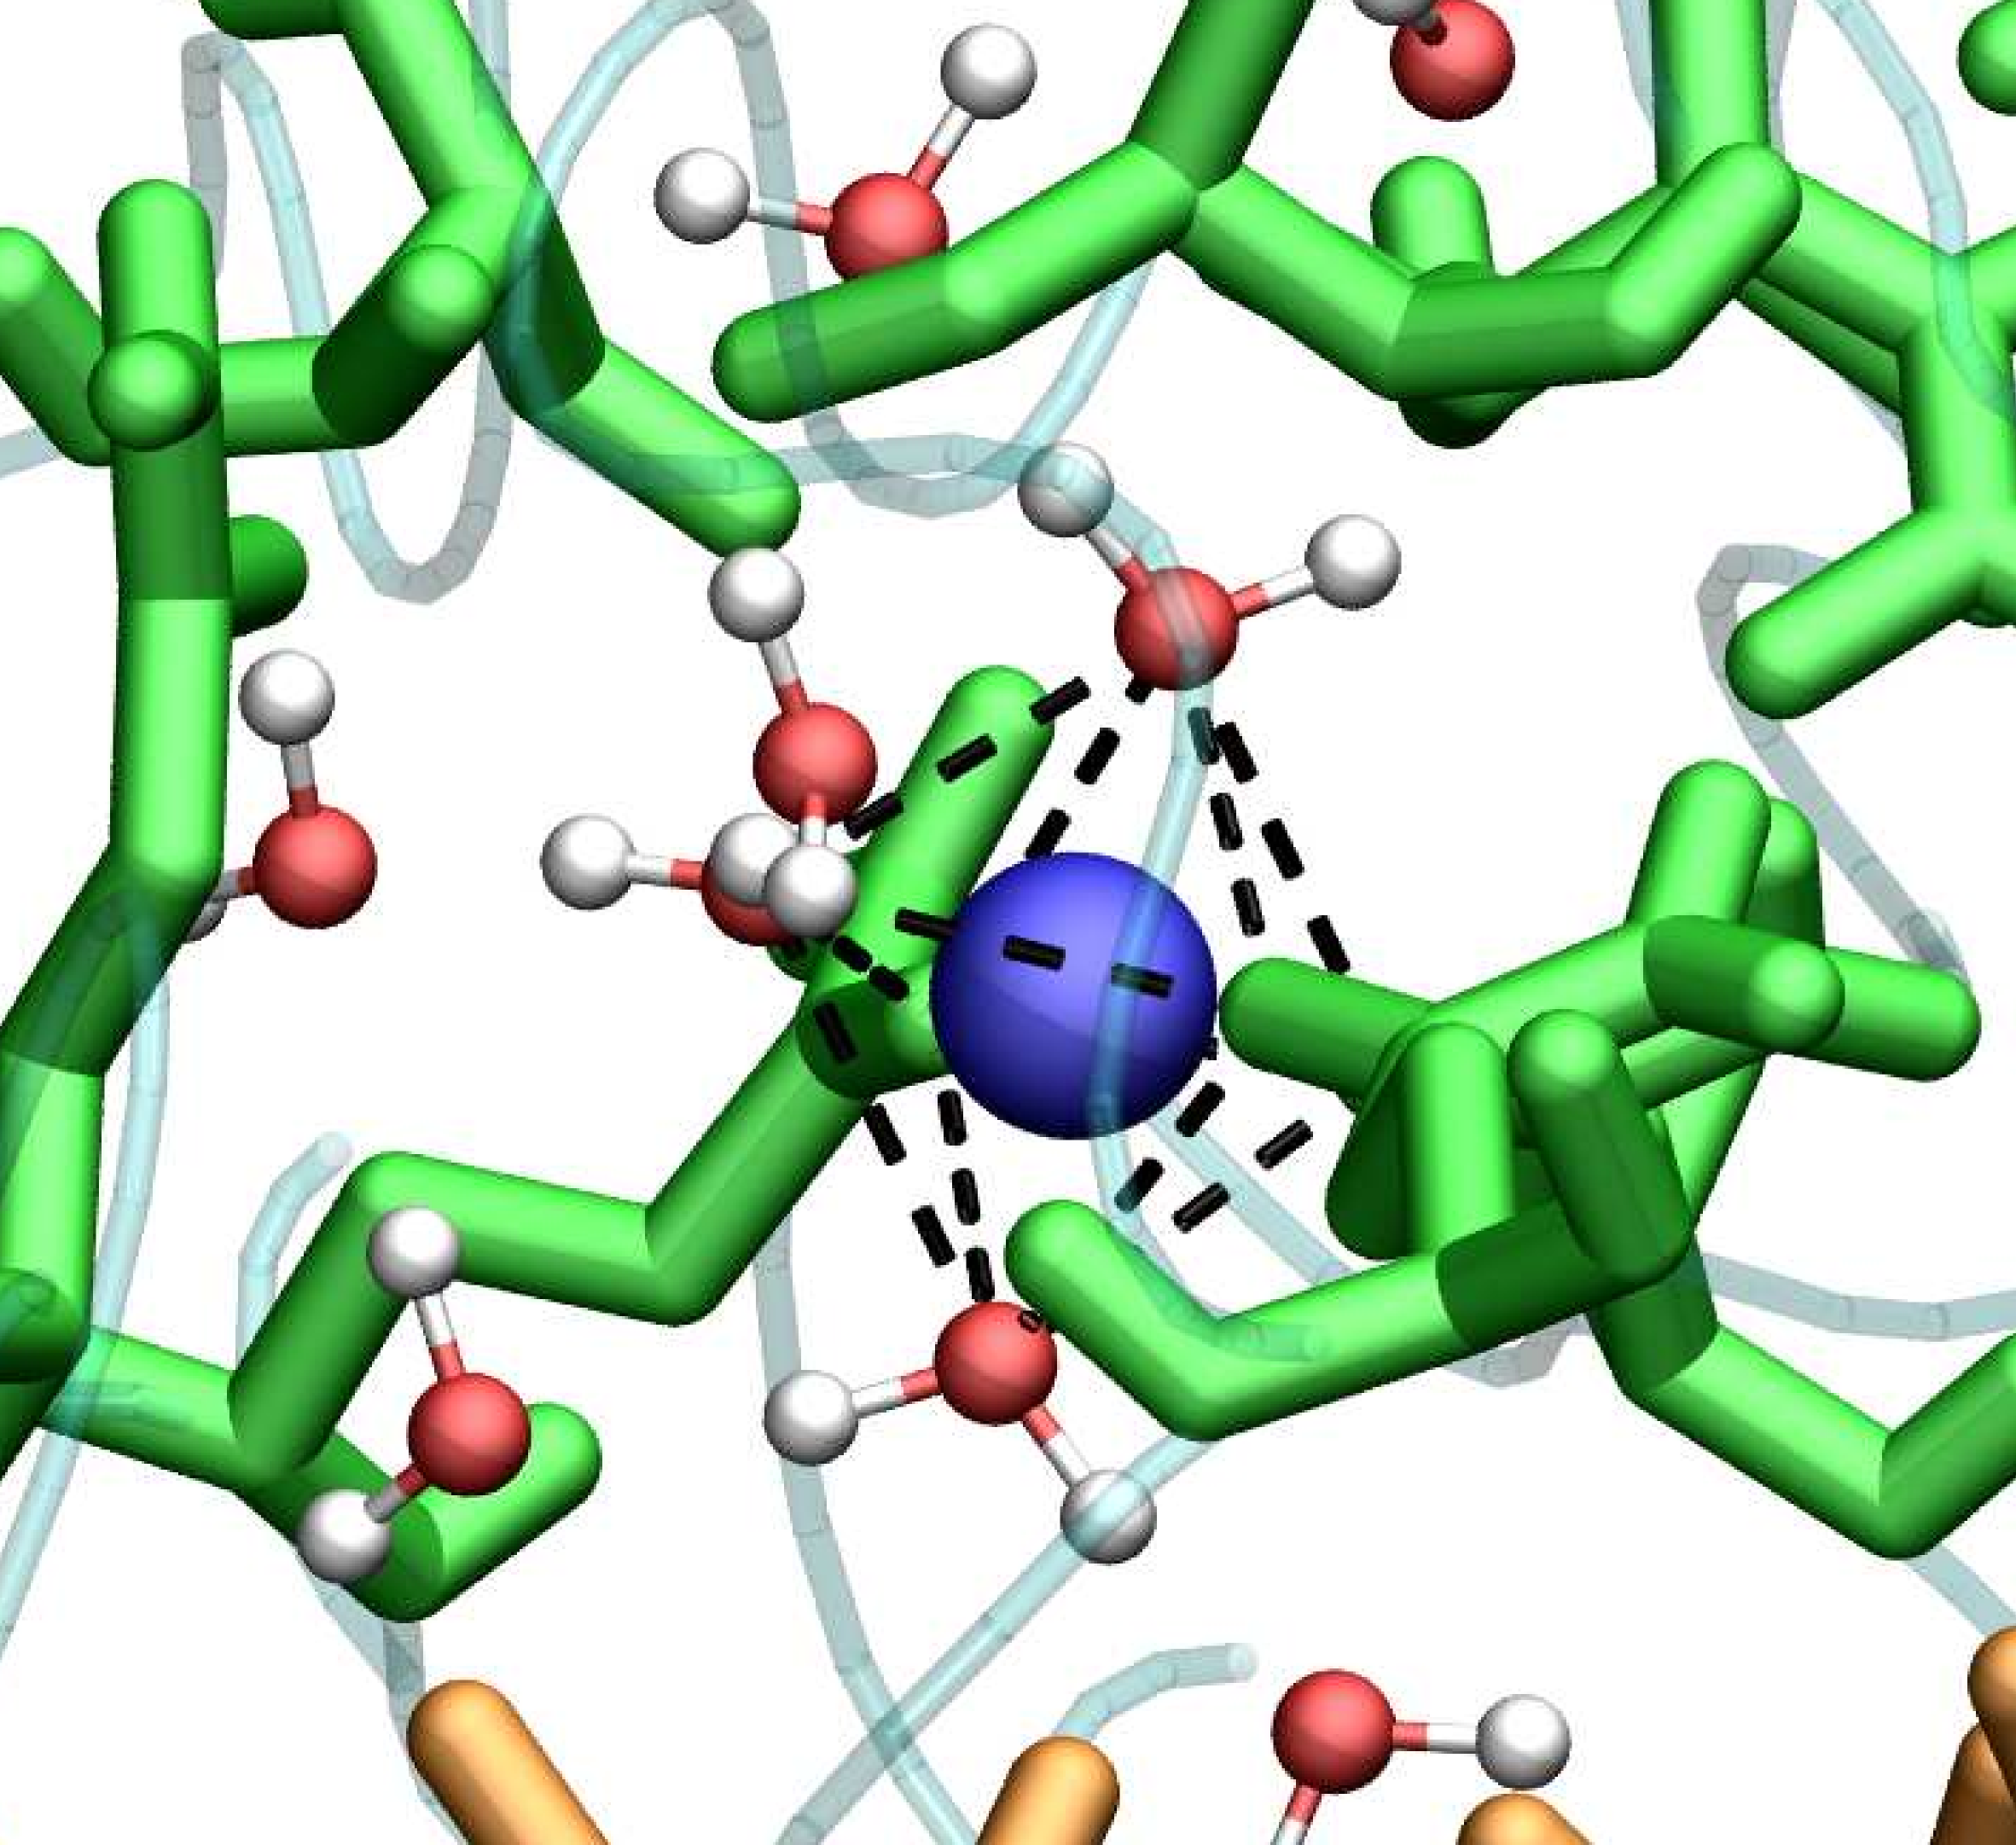
\includegraphics[width=0.8\textwidth]{Figure/mg_sol.png}
\end{column}
\end{columns}
\end{frame}

\begin{frame}
\centering
\Large !`Muchas Gracias!
\end{frame}

\begin{frame}[t]{Agradecimientos}
\small
\begin{itemize}
    \item<1-> Al departamento de Física de la UNS y al Instituto de Física del Sur por formarme y darme los medios para realizar este doctorado.
    \item<2-> A mi director, \textbf{Marcelo}, por introducirme en el mundo de la investigación.
    \item<3-> A mis compañeros de oficina, que me soportaron todo el doctorado. A \textbf{Fernando} que me enseño todo lo que sabia y me ayudo en los primeros pasos de este viaje.
    \item<4-> A \textbf{Nestor}, por sus charlas de ciencia, educación y otros temas.
    \item<5-> A \textbf{Sebastian} y \textbf{Michellina}, que me ayudaron y formaron como docente. A todos los integrantes de Curiosos. A todos los compañeros de cátedra.
    \item<6-> A \textbf{Ilan} y \textbf{Nadia} por transitar este camino juntos y ayudarnos mutuamente aunque sea solo prestando la oreja. A todos los que pasaron por la ofícina de becarios.
    \item<7-> A mis amigos de la universidad, \textbf{Duilio}, \textbf{Pau}, \textbf{Cris} y \textbf{Licho}, por su amistad y por aguantarme en todo este viaje.
    \item<8-> A \textbf{Maju}, hicimos todo este camino juntos y no se si lo hubiera terminado sin su amistad.
    \item<9-> A mis amigos de la infancia, \textbf{Rober}, \textbf{Seba}, \textbf{Gaspar}, \textbf{Fede} y \textbf{Sonia}, después de
tanto tiempo siempre presentes.
    \item<10-> Por último y más importante a mi \textbf{Familia}. A mis \textbf{Padres} por darme todo. A mis
\textbf{Hermanos}, a pesar de las peleas, siempre apoyándome.
    \item<11-> A \textbf{Jobo}.
\end{itemize}
\end{frame}

\end{document}